\section{Sperimentazione sui pannelli reali}
Come anticipato, al fine di valorizzare maggiormente i risultati ottenuti in
questo progetto, si 
è deciso di procedere con lo studio di dati reali, relativi alla \textit{phase
  3} del \textbf{1000
  Genome
  Project}\footnote{\url{https://ftp.1000genomes.ebi.ac.uk/vol1/ftp/release/20130502/}}
\cite{1kgp}.\\ 
Tali pannelli, disponibili in formato \textit{VCF}, presentano un numero
costante di sample, ovvero 5008, mentre a variare è il numero di siti. Essendo
dati reali, non si ha la sola presenza di siti biallelici. Si è quindi proceduto
alla selezione dei soli siti biallelici, ottenendo quindi pannelli costruiti su
un alfabeto binario $\Sigma=\{0,1\}$, tramite l'uso di \textbf{bcftools}
\cite{bcftools}, tramite il comando \texttt{bcftools view -m2 -M2
  -v snps}.\\
La prima selezione dei pannelli è stata dettata dalla volontà di studiare, per
praticità, matrici non troppo estese. Si sono, quindi, scelti i pannelli
relativi:
\begin{itemize}
  \item al cromosoma 22, con 1055454 siti
  \item al cromosoma 20, con 1739315 siti
  \item al cromosoma 18, con 2171378 siti
  \item al cromosoma 16, con 2596072 siti
\end{itemize}
In aggiunta, si è studiato uno dei pannelli più grossi disponibili, ovvero
quello relativo al cromosoma 1, con 6196151 siti.\\
Al fine del computo degli SMEM, avendo un numero ridotto di sample a
disposizione, si è scelto di estrarre da ognuno 100 sample da usare come
query.\\
Prima di procedere con l'effettivo studio delle performance di calcolo degli
SMEM, trattandosi di pannelli reali, è risultata interessante una preliminare
indagine esplorativa sulla natura di tali pannelli in termini di
\textit{sparsità} degli alleli e di conseguente numerosità delle run. Si è
quindi calcolato, per i cinque pannelli, il numero di simboli $\sigma=0$ e
$\sigma=1$, notando come il numero di simboli $\sigma=1$ fosse molto ridotto
rispetto al totale, essendo il $\sim 0.03\%$ del totale dei simboli. Una tale
sparsità del dato si ``propaga'' anche sul numero di run di ogni colonna, avendo
di fatto pochi simboli $\sigma=1$ in ogni colonna, simboli che possono anche
essere nella medesima run dopo la permutazione data dalla
\textit{PBWT}. Si ricordi, inoltre, che tale permutazione, come per la
\textit{BWT}, è studiata per essere 
maggiormente efficiente nel caso del dato biologico. Studiando, quindi, il
numero medio di run per colonna e il numero 
massimo di run in una colonna si è confermato tale risultato, infatti:
\begin{itemize}
  \item per il cromosoma 22 si ha un numero medio di 14 run, con un massimo di
  2450
  \item per il cromosoma 20 si ha un numero medio di 11 run, con un massimo di
  2176
  \item per il cromosoma 18 si ha un numero medio di 11 run, con un massimo di
  2365
  \item per il cromosoma 16 si ha un numero medio di 12 run, con un massimo di
  2330
  \item per il cromosoma 1 si ha un numero medio di 11 run, con un massimo di
  2721 
\end{itemize}
Si conferma quindi il risultato atteso, risultato che è a favore, in termini di
complessità in spazio, della \textit{RLPBWT} in quanto tutte le componenti sono
proporzionali al numero di run. In figura \ref{fig:chrrun} si riportano
graficamente tali risultati.
\begin{figure}
  \centering
  \begin{subfigure}{.45\textwidth}
    \centering
    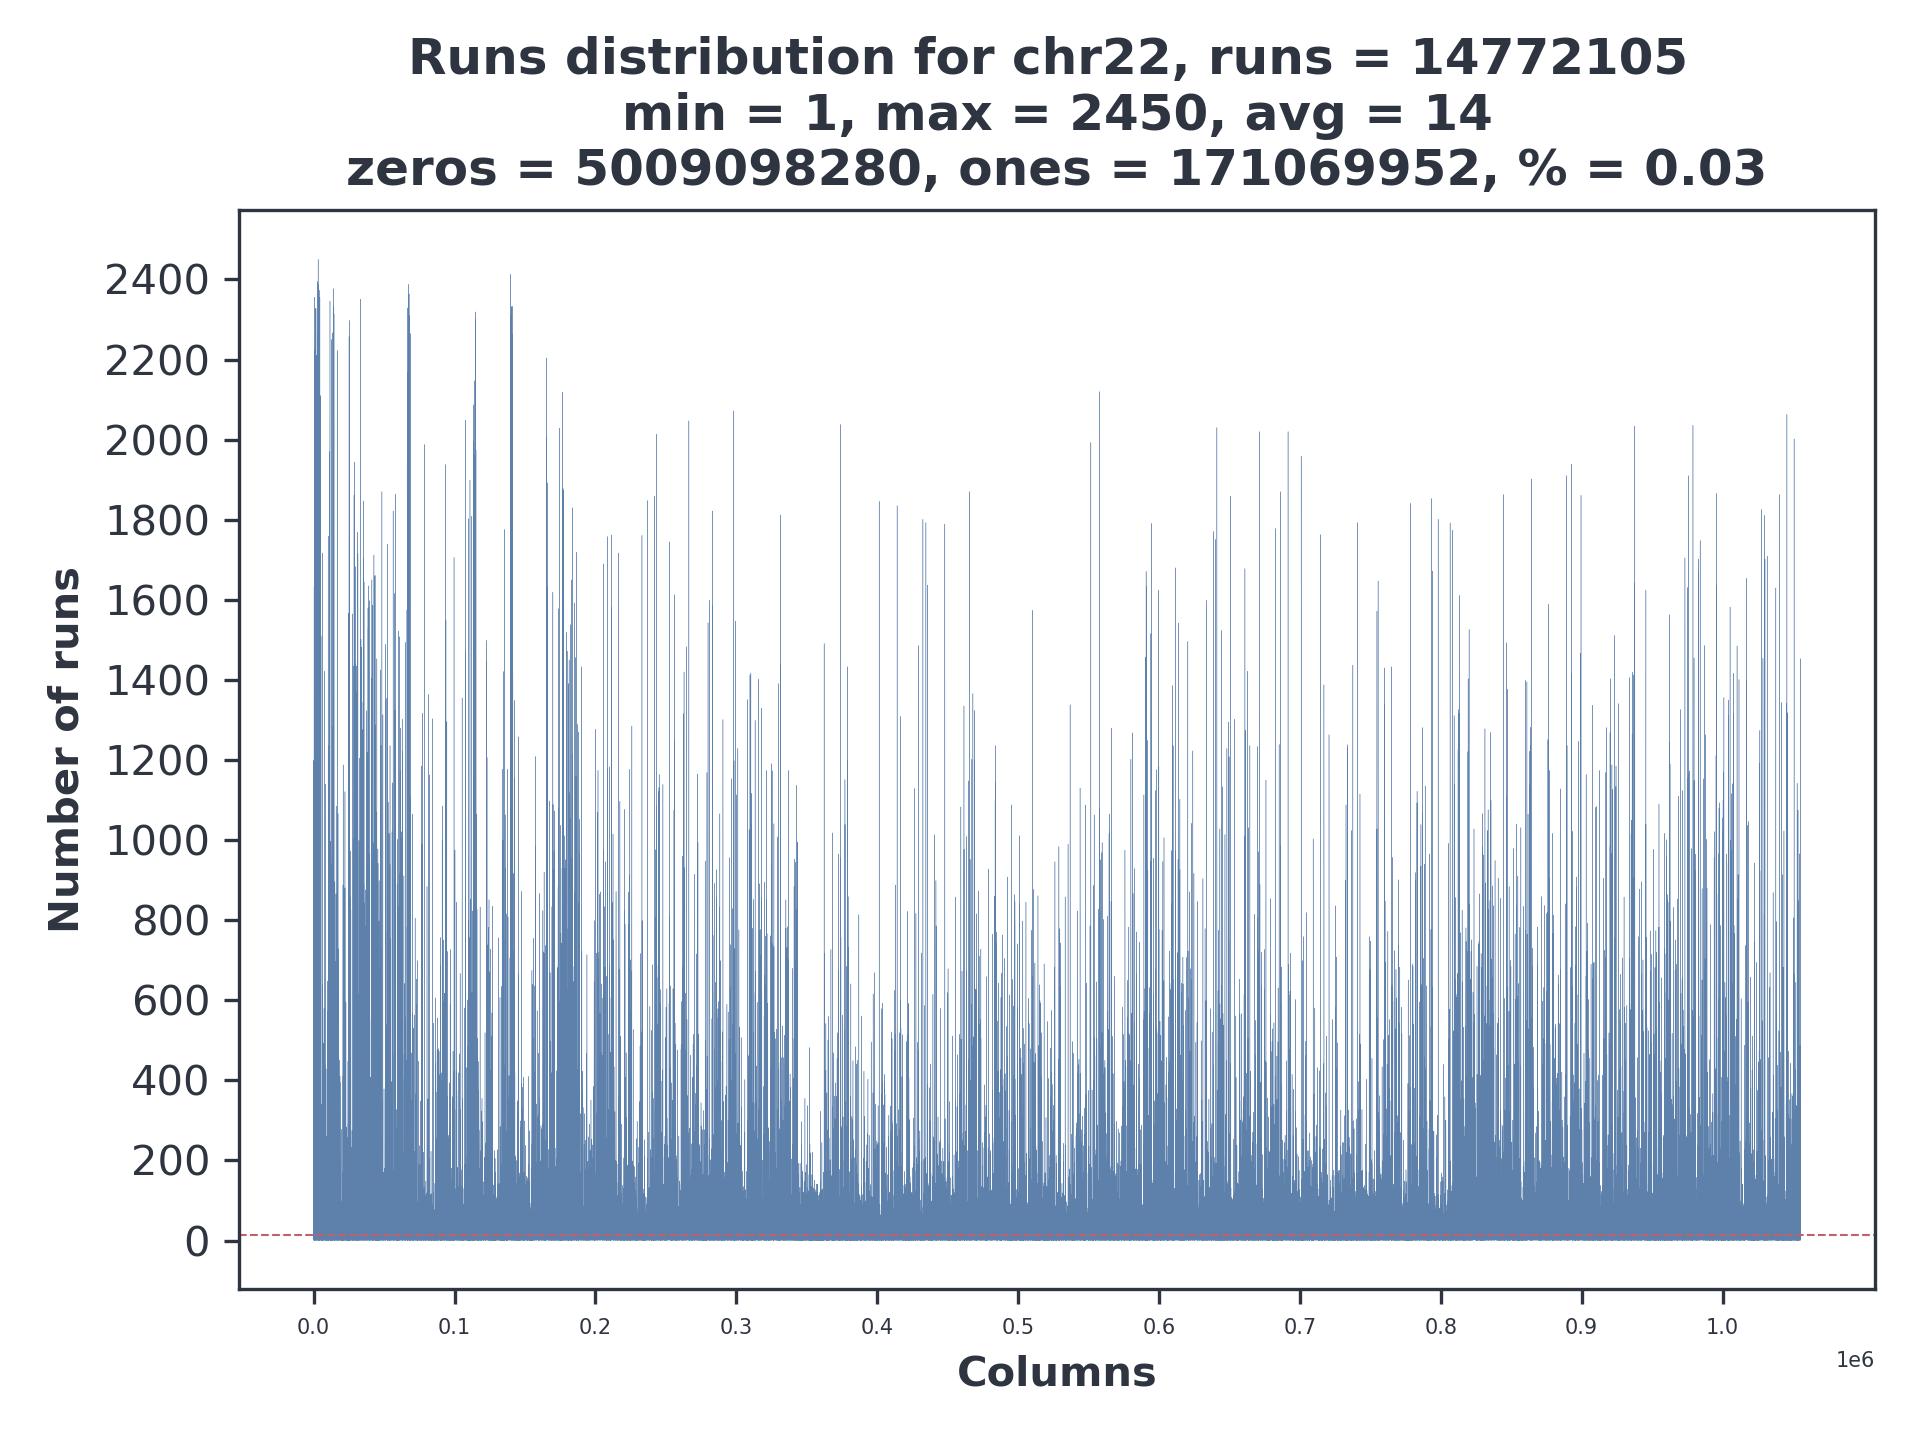
\includegraphics[width=\linewidth]{img/22_runs.png}
  \end{subfigure}%
  \begin{subfigure}{.45\textwidth}
    \centering
    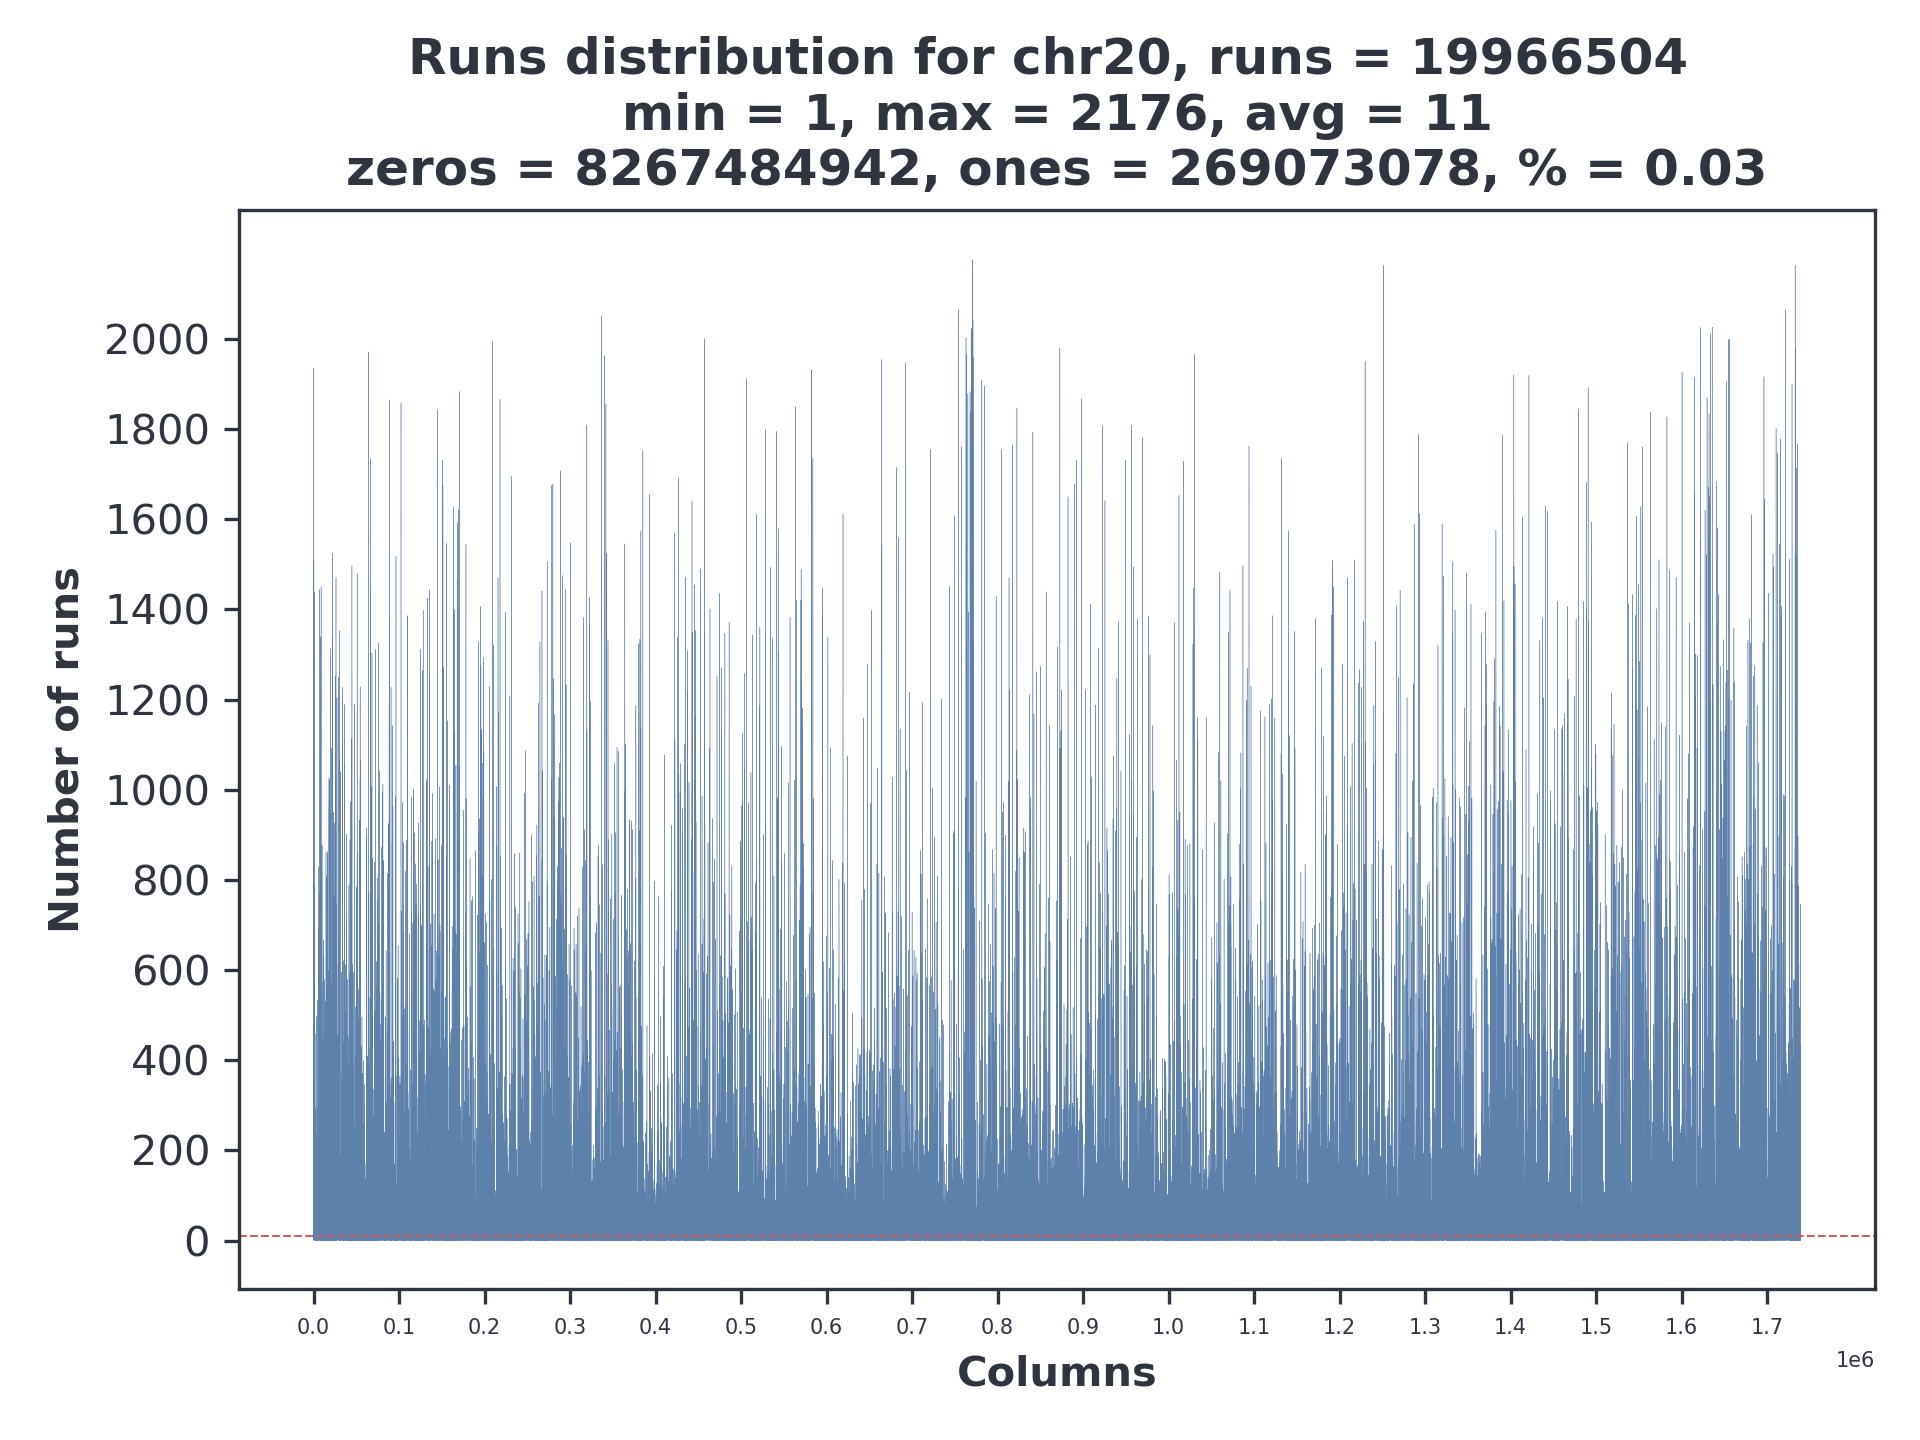
\includegraphics[width=\linewidth]{img/20_runs.png}
  \end{subfigure}
  \begin{subfigure}{.45\textwidth}
    \centering
    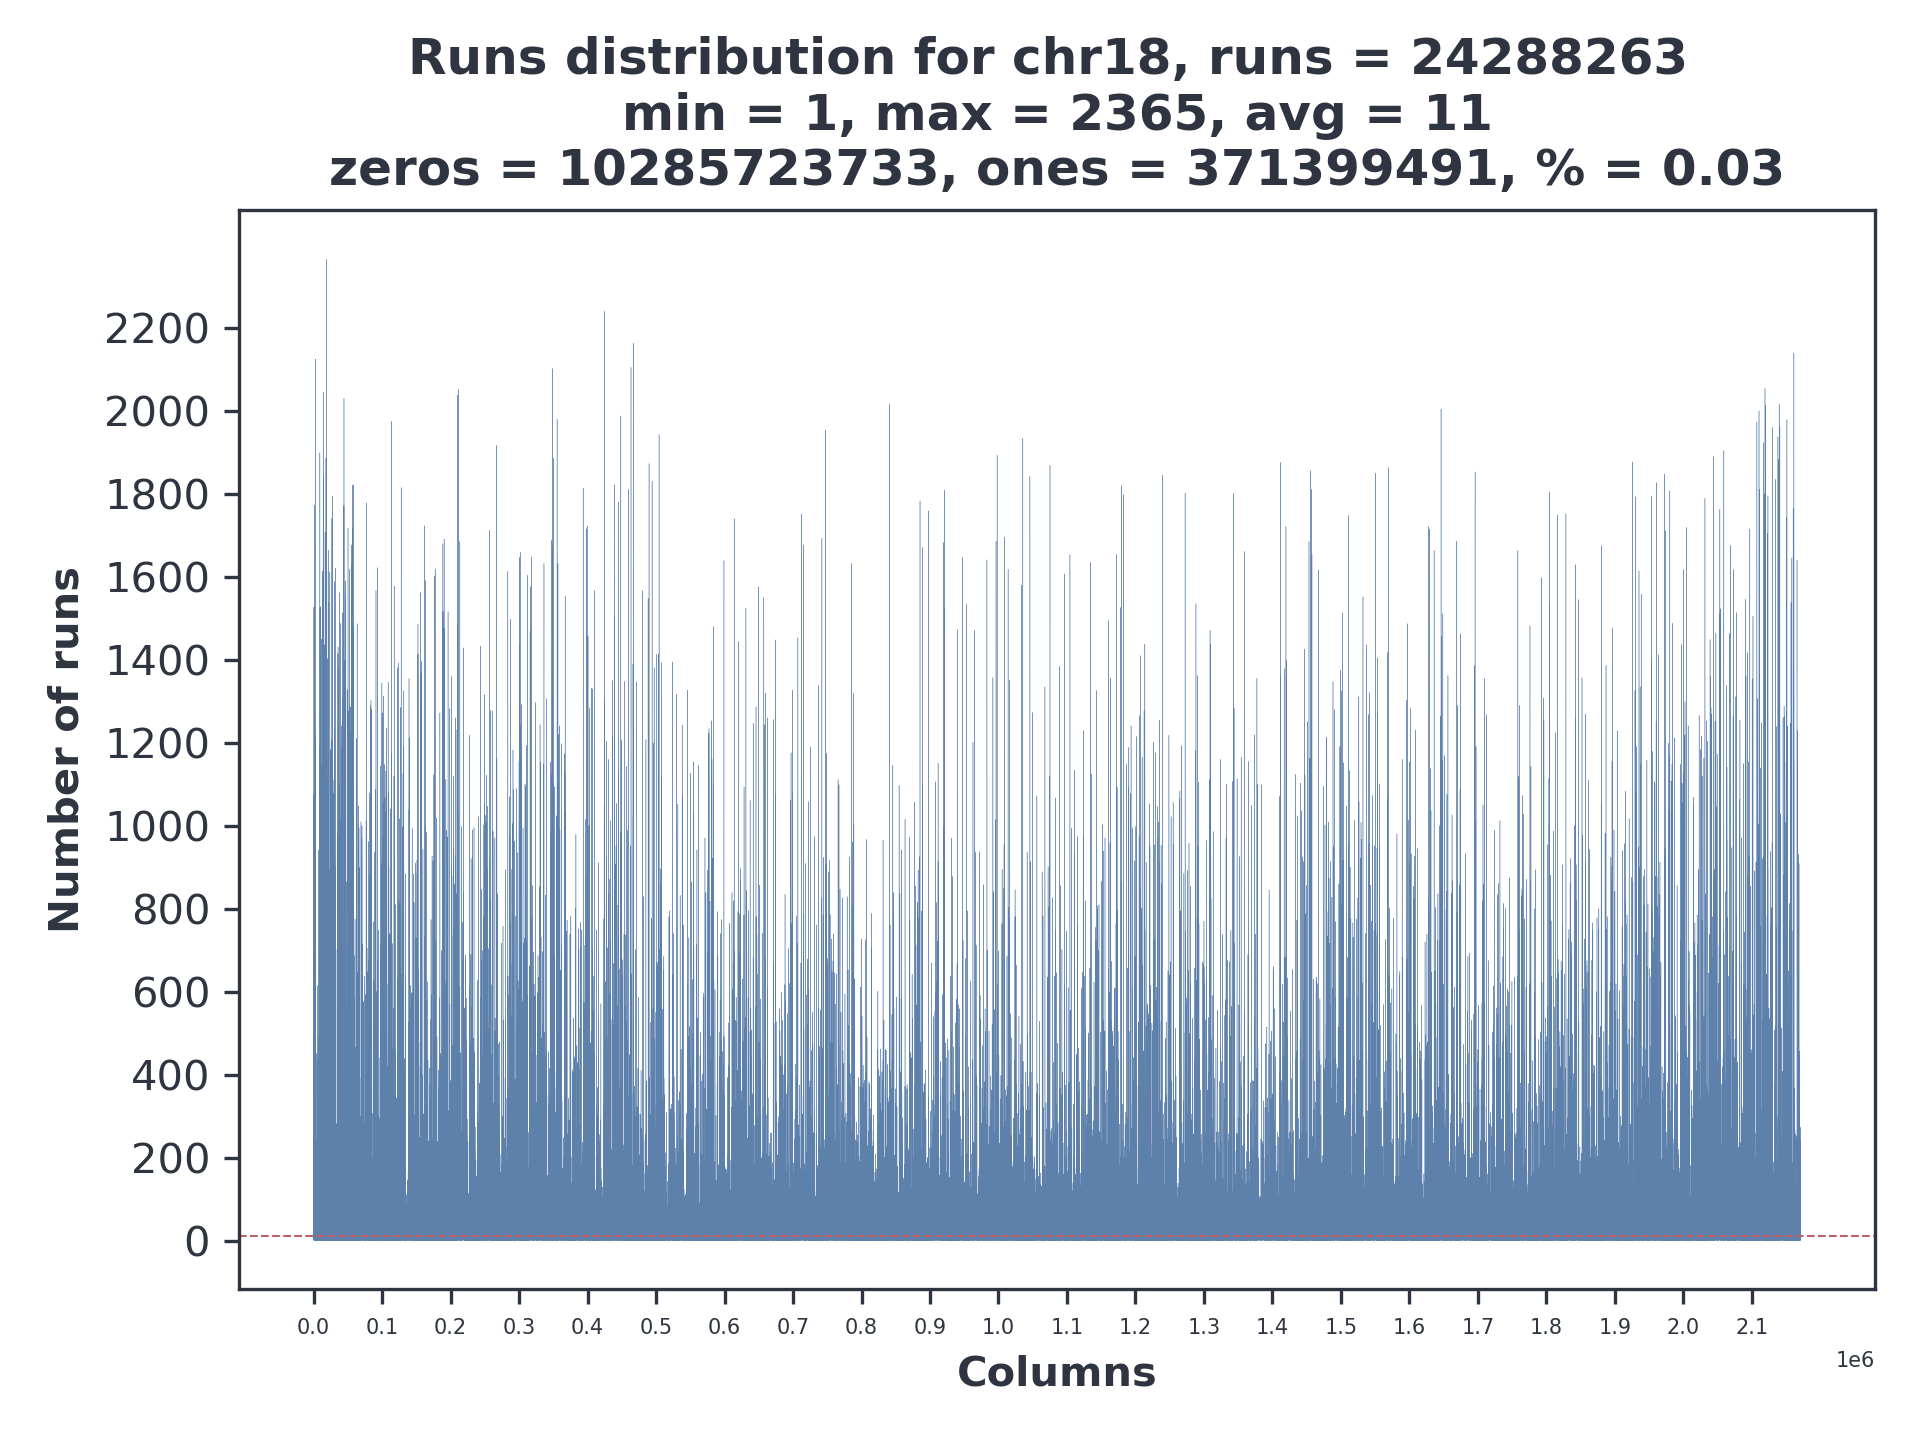
\includegraphics[width=\linewidth]{img/18_runs.png}
  \end{subfigure}%
  \begin{subfigure}{.45\textwidth}
    \centering
    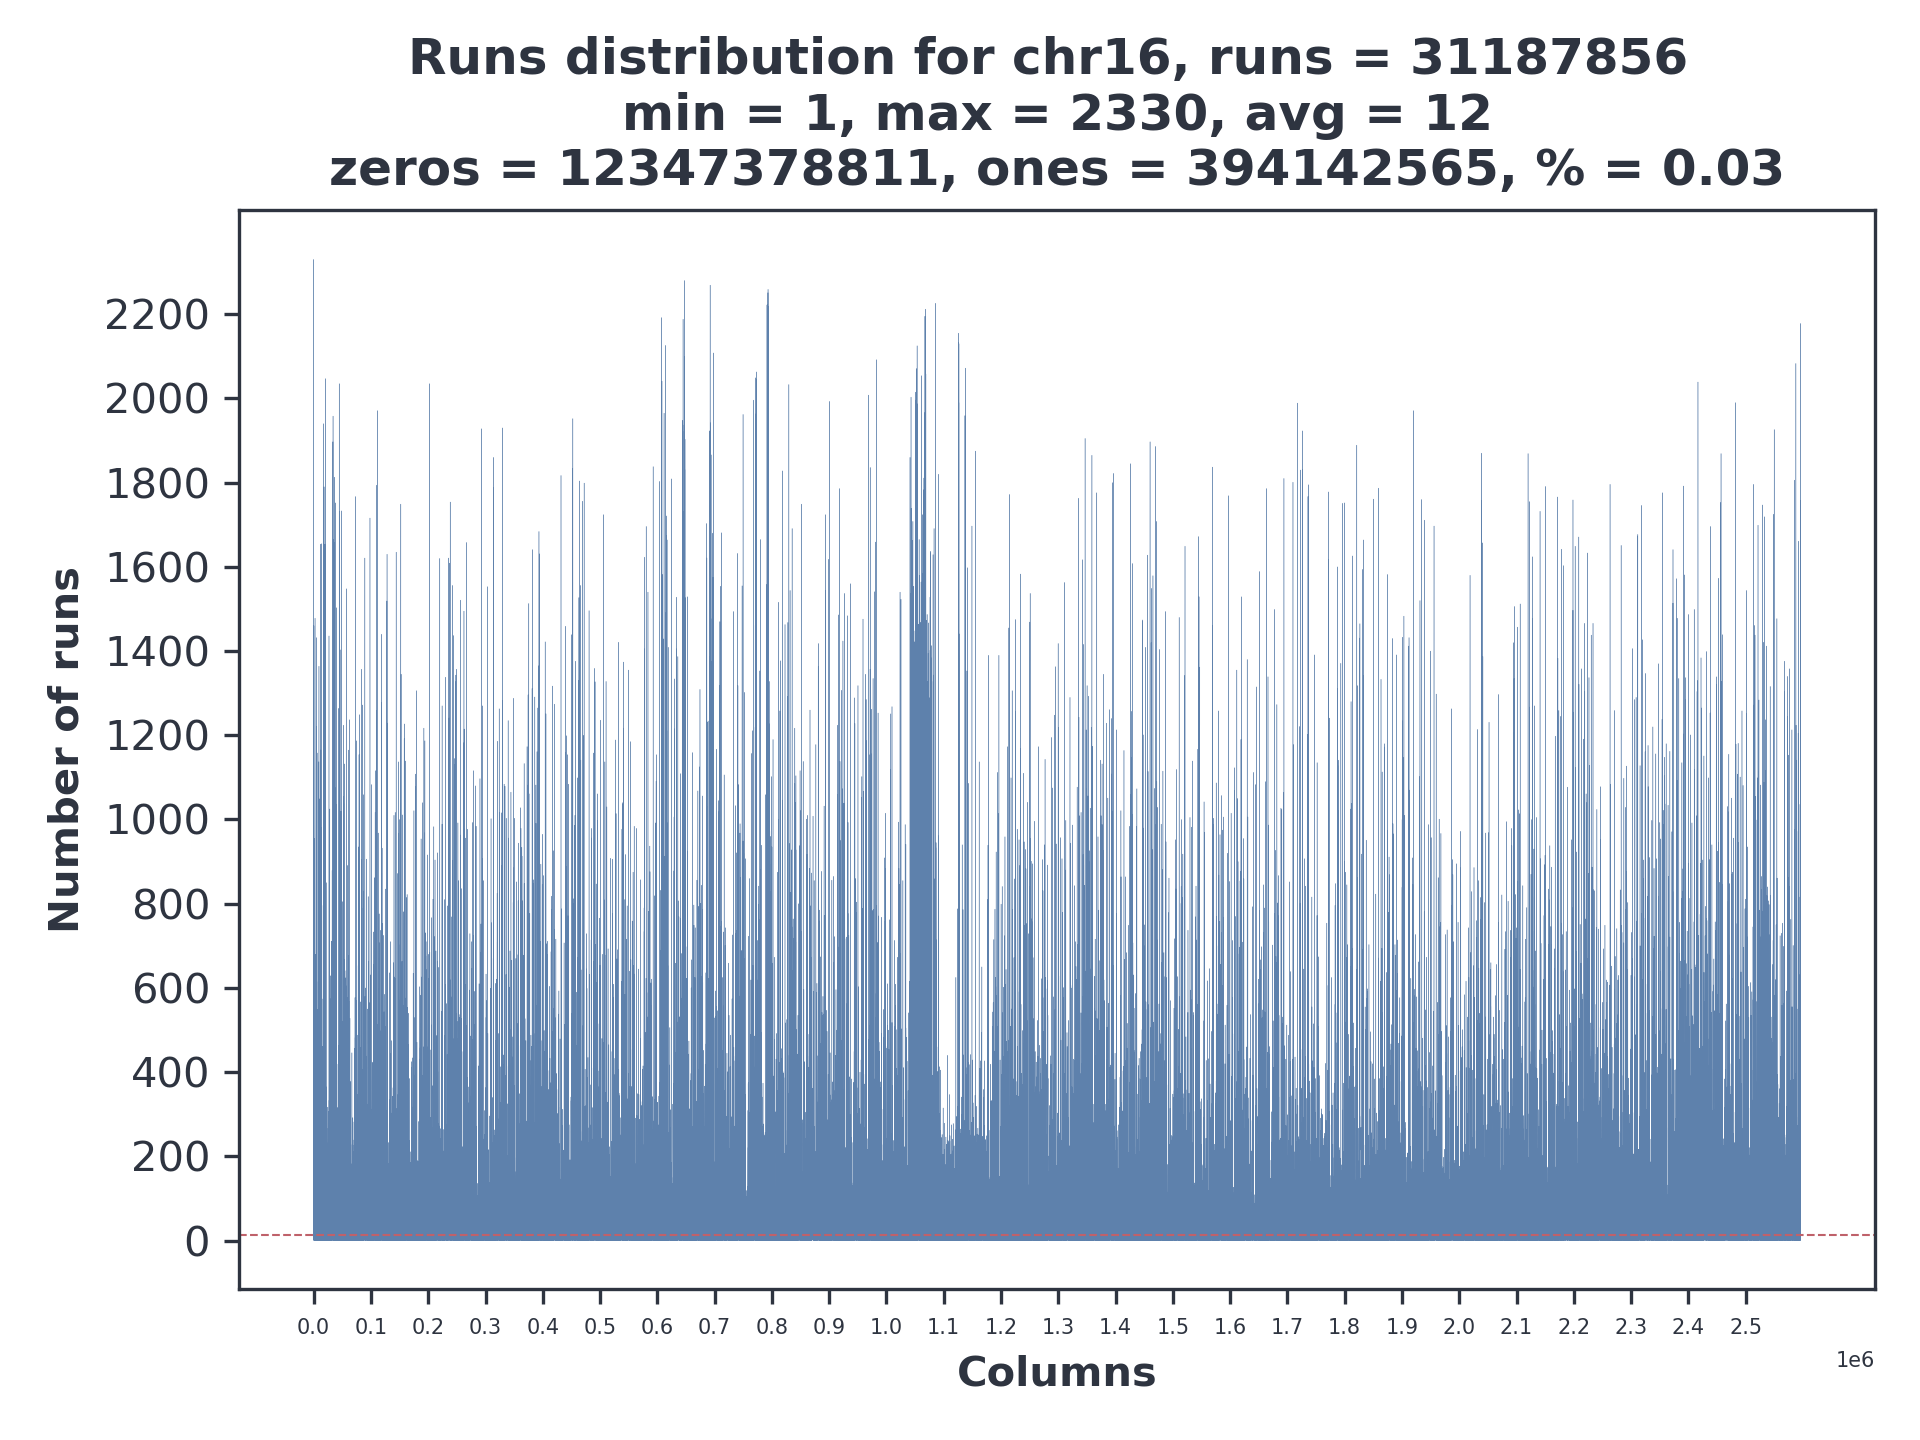
\includegraphics[width=\linewidth]{img/16_runs.png}
  \end{subfigure}
  \begin{subfigure}{.45\textwidth}
    \centering
    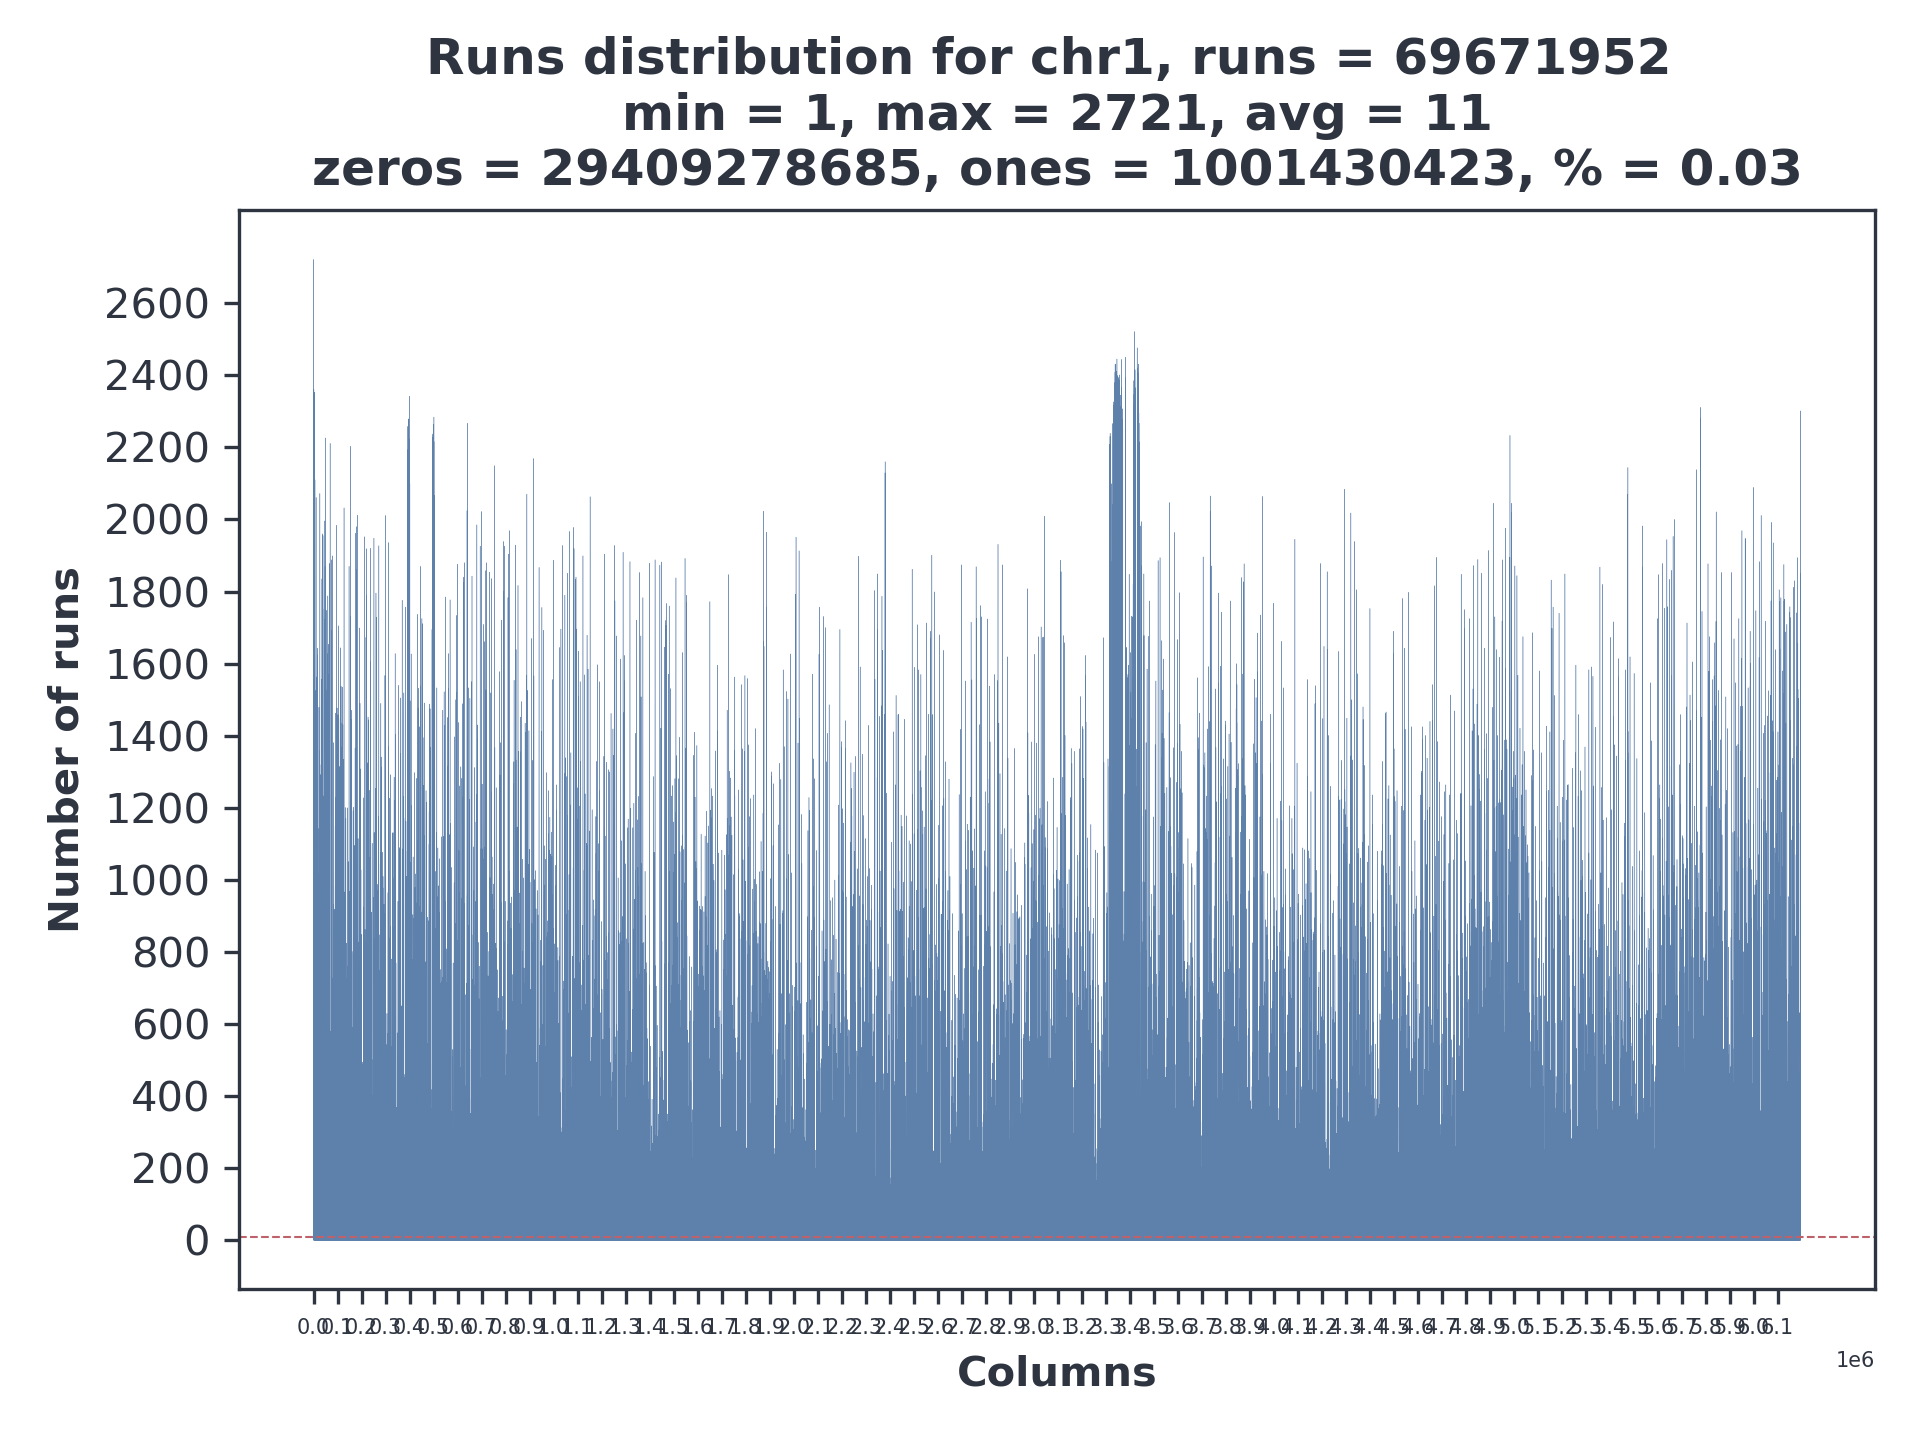
\includegraphics[width=\linewidth]{img/1_runs.png}
  \end{subfigure}
  \caption{Distribuzione delle run per colonna con il numero
    minimo/medio/massimo delle stesse. Nel titolo si hanno anche il numero
    complessivo di run, il numero di simboli $\sigma=0$ e $\sigma=1$, nonché la
    percentuale della quantità di questi ultimi sul totale dei simboli.}
  \label{fig:chrrun}
\end{figure}

Viste le dimensioni di tali pannelli si ritiene necessario studiare, dal punto
di vista del tempo macchina e dei picchi di memoria necessaria, i vari step
della sperimentazione:
\begin{itemize}
  \item la fase di \textit{preprocessing}, necessaria per la \textit{RLPBWT},
  comprendente: 
  \begin{itemize}
    \item la conversione dei file VCF in file MACs
    \item l'estrazione del pannello delle query e la creazione del nuovo
    pannello di reference
    \item la produzione dell\textit{SLP} del pannello di reference, comprendente
    sia la produzione della stringa che l'esecuzione di \textit{BigRepair} che
    di \textit{ShapedSlp}
  \end{itemize}
  \item la costruzione delle varianti della \textit{RLPBWT} e dei file ad hoc
  per la \textit{PBWT}
  \item il calcolo degli SMEMs
\end{itemize}
In generale i risultati ottenuti risultano essere coerenti con quanto visto nei
pannelli simulati.
\paragraph{Preprocessing}
In figura \ref{fig:prechr} si possono analizzare le prestazioni delle tre
fasi. La separazione del pannello con le query risulta essere assolutamente
ininfluente e, di fatto, anche la conversione tra i due formati (conversione che
diventerebbe non necessaria implementando l'input direttamente da file VCF) non
necessita particolari considerazioni. Bisogna, però, analizzare la costruzione
dell'\textit{SLP}. Per quanto quest'operazione sia da svolgersi \textit{una
  tantum}, le richieste in termini di memoria sono nell'ordine delle centinaia
di gigabytes di RAM mentre i tempi di calcolo sono nell'ordine delle
ore. D'altro canto, bisogna considerare che tutti gli algoritmi per la produzione
dell'\textit{SLP} sono studiati per partire da una singola stringa e non da una
matrice e questo potrebbe lasciar spazio a diverse ottimizzazioni. Inoltre
questa fase è necessaria solo per due delle tre soluzioni studiate per la
\textit{RLPBWT} e, come già detto, il fatto che sia necessaria solo una volta
deve essere preso in considerazione nell'ottica di un confronto con, ad esempio,
lo spazio richiesto dall'\textit{algoritmo 5} di Durbin, che richiede $13NM$
bytes ad ogni esecuzione.
\begin{figure}
  \centering
  \begin{subfigure}{.5\textwidth}
    \centering
    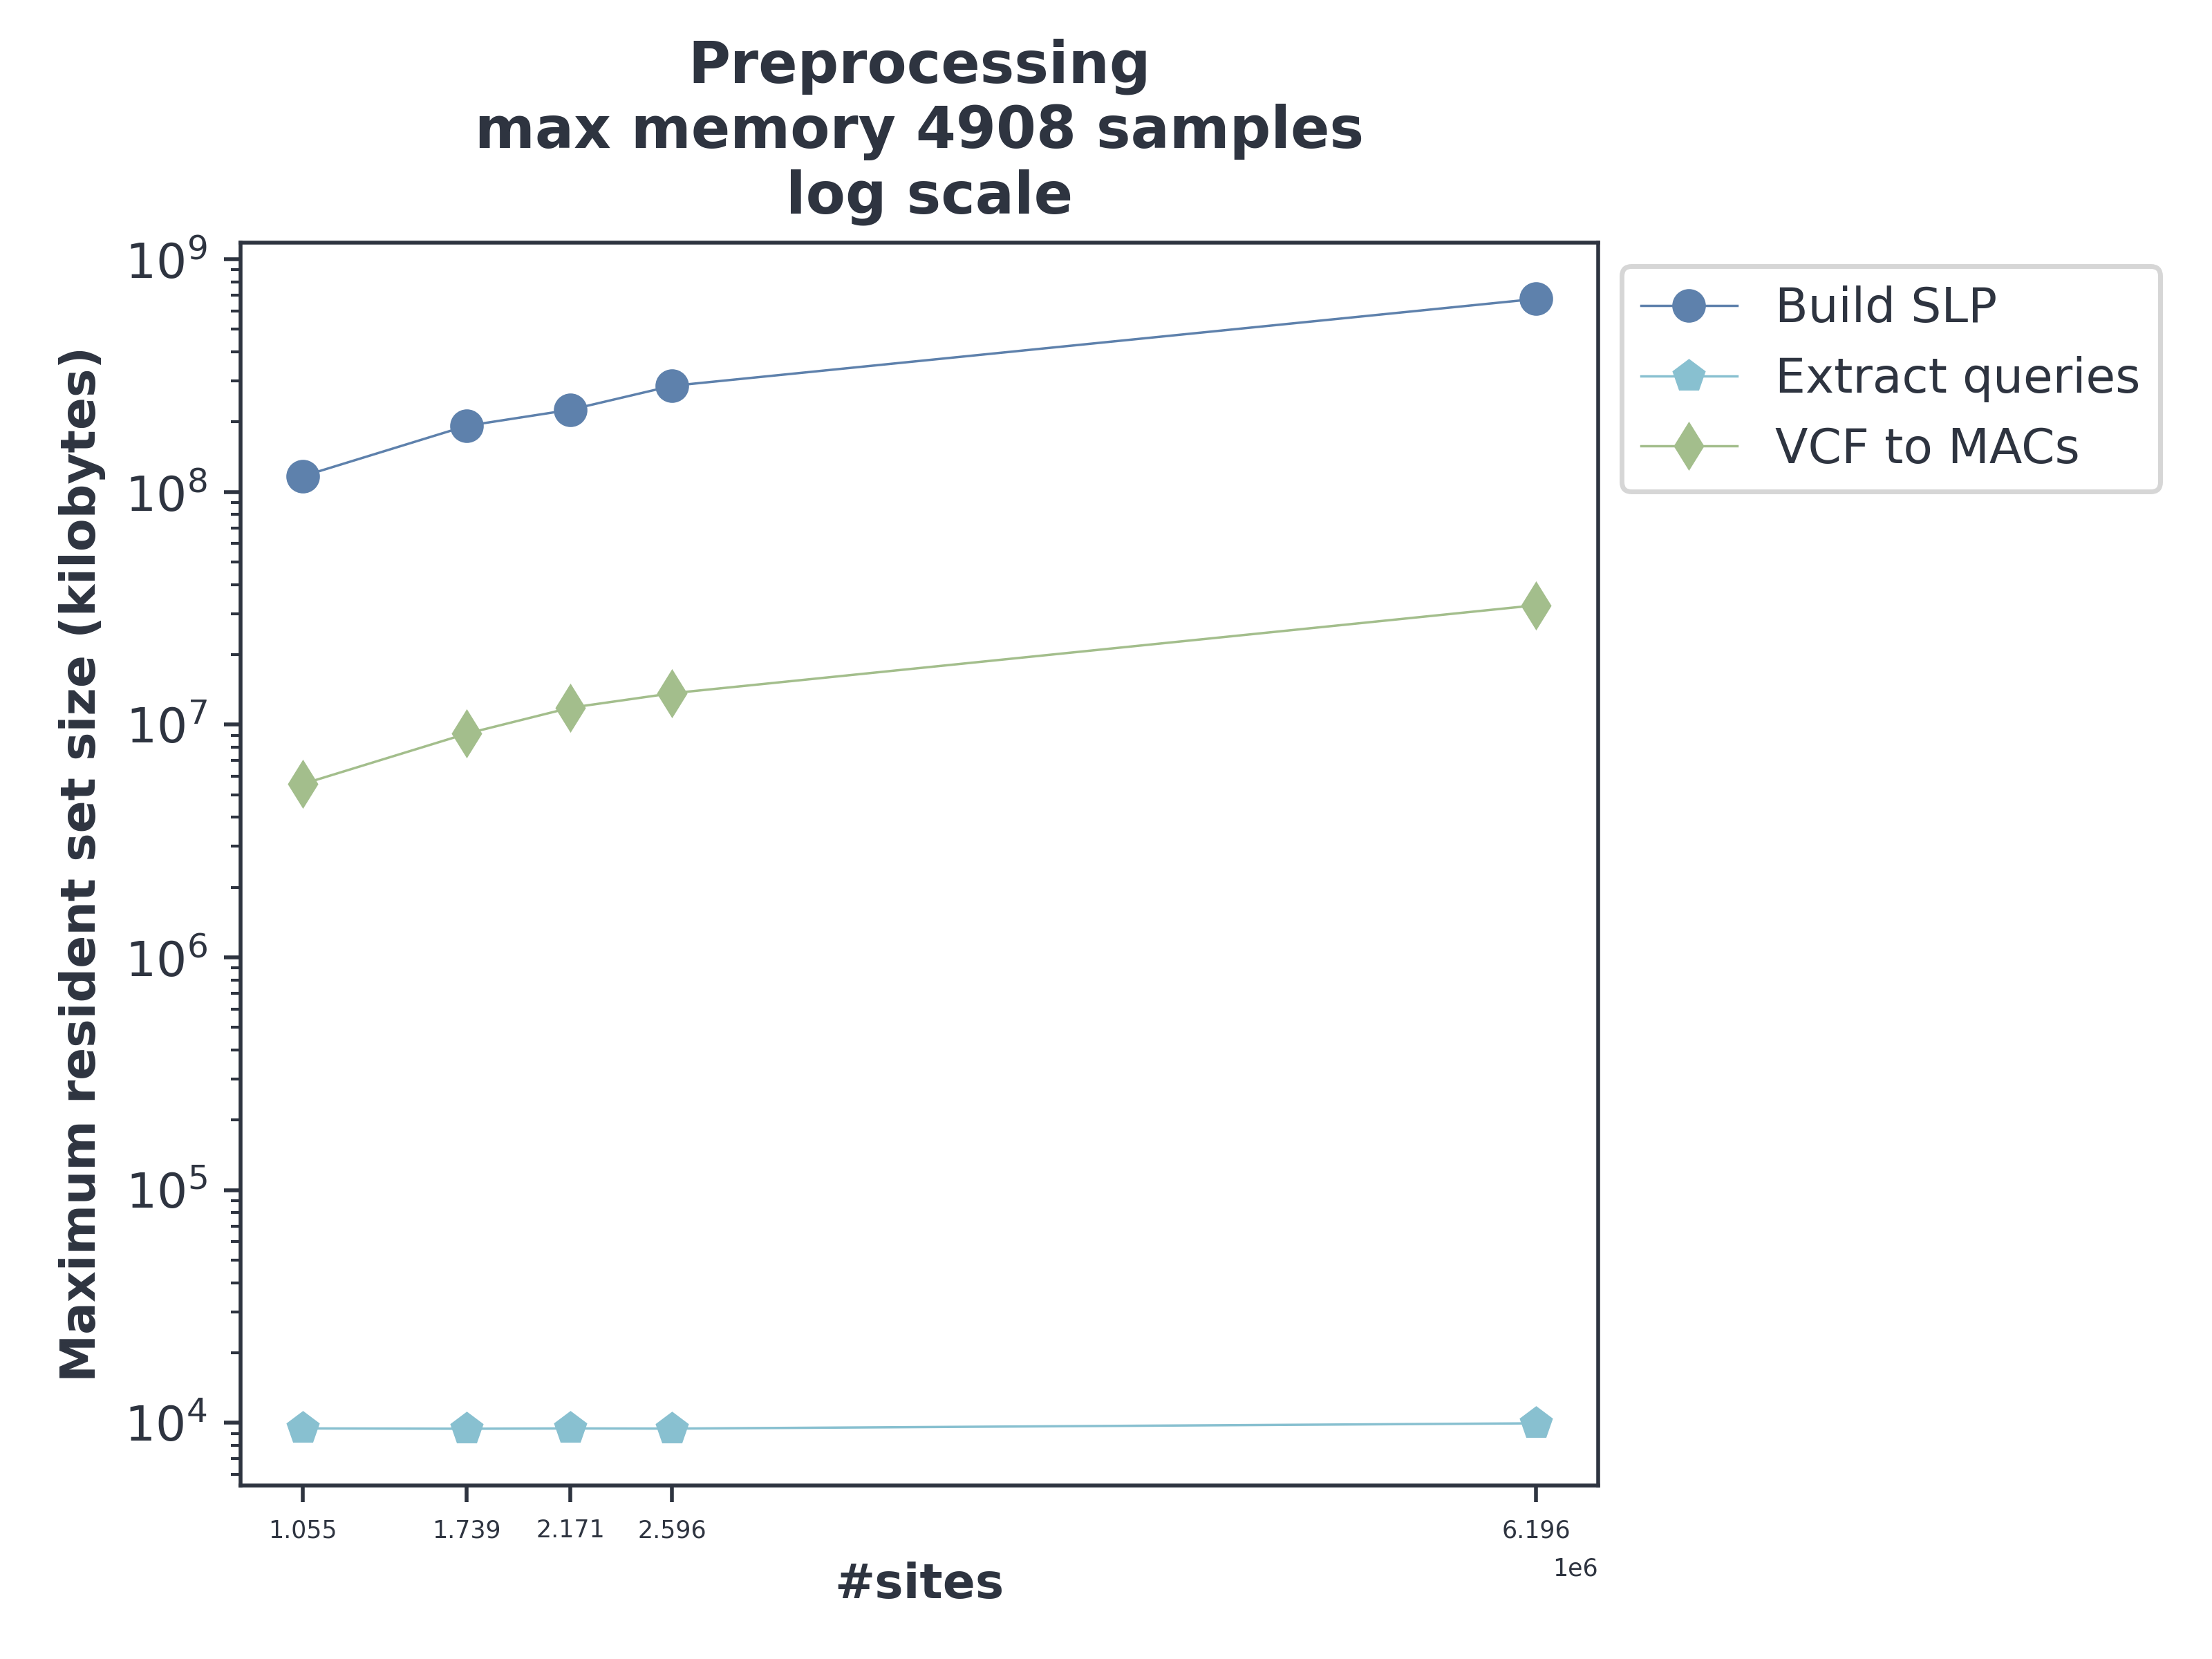
\includegraphics[width=\linewidth]{img/pre_mem_log.png}
  \end{subfigure}%
  \begin{subfigure}{.5\textwidth}
    \centering
    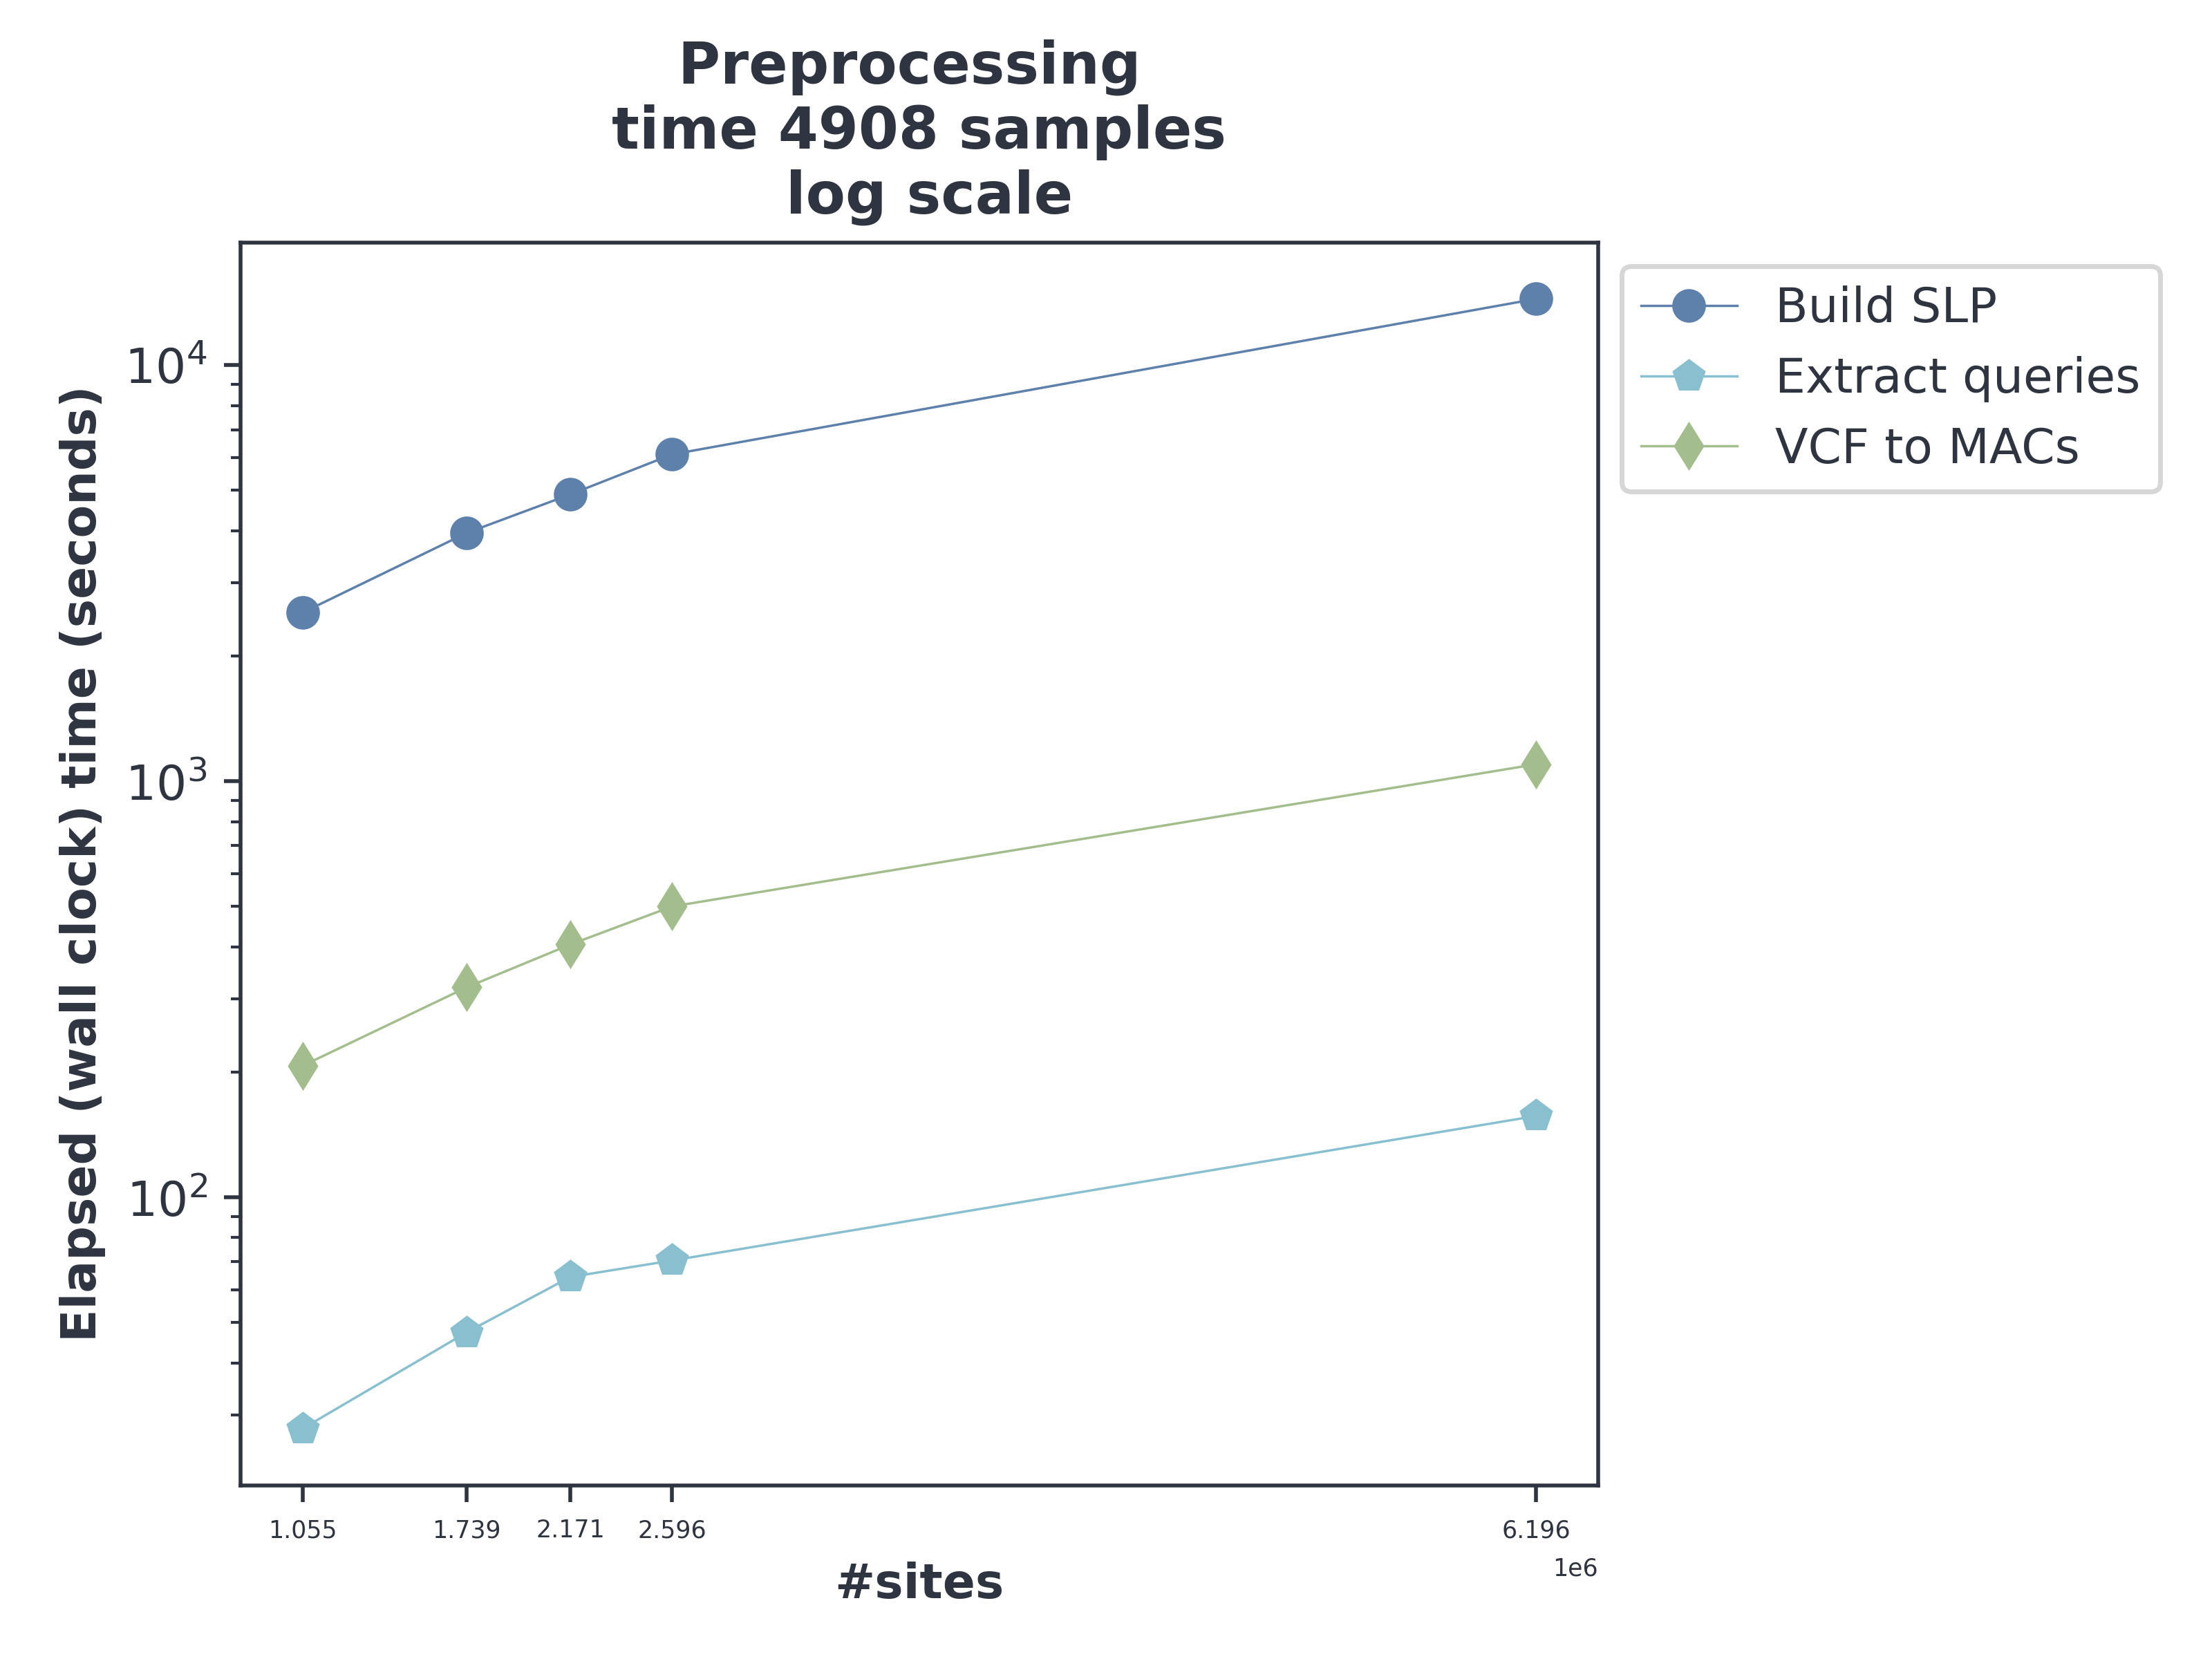
\includegraphics[width=\linewidth]{img/pre_time_log.png}
  \end{subfigure}
  \caption{Tempo richiesto e picco di memoria, in scala logaritmica, per le
    tre fasi di preprocessing 
    dei dati in input per la \textit{RLPBWT}.}
  \label{fig:prechr}
\end{figure}

In figura \ref{fig:slpmacschr} si può osservare il vantaggio in termini di
memoria che si ha con l'uso degli \textit{SLP}, confrontando il peso dei file
MACs con il peso delle grammatiche compresse. Di seguito si possono confrontare
quantitativamente tali risultati, che risultano percentualmente peggiori
rispetto a quanto visto coi pannelli simulati:
\begin{table}[H]
  \centering
  \begin{tabular}{c|c|c|c|c}
    \textbf{\#Samples} & \textbf{\#Siti} & \textbf{SLP (\textit{kb})}
    & \textbf{MACs (\textit{kb})} & \textbf{\%}\\
    \hline
    4908 & 1055454 & 45866.4 & 5079359.44 & 0.9\\
    4908 & 1739315 & 63378.56 & 8370121.94 & 0.76\\
    4908 & 2171378 & 82088.5 & 10449409.15 & 0.79\\
    4908 & 2596072 & 101095.88 & 12493108.91 & 0.81\\
    4908 & 6196151 & 232363.65 & 29821949.72 & 0.78\\
  \end{tabular}
\end{table}
Nonostante tale peggioramento la potenza di compressione degli \textup{SLP}
risulta comunque non trascurabile.
\begin{figure}
  \centering
  \begin{subfigure}{.5\textwidth}
    \centering
    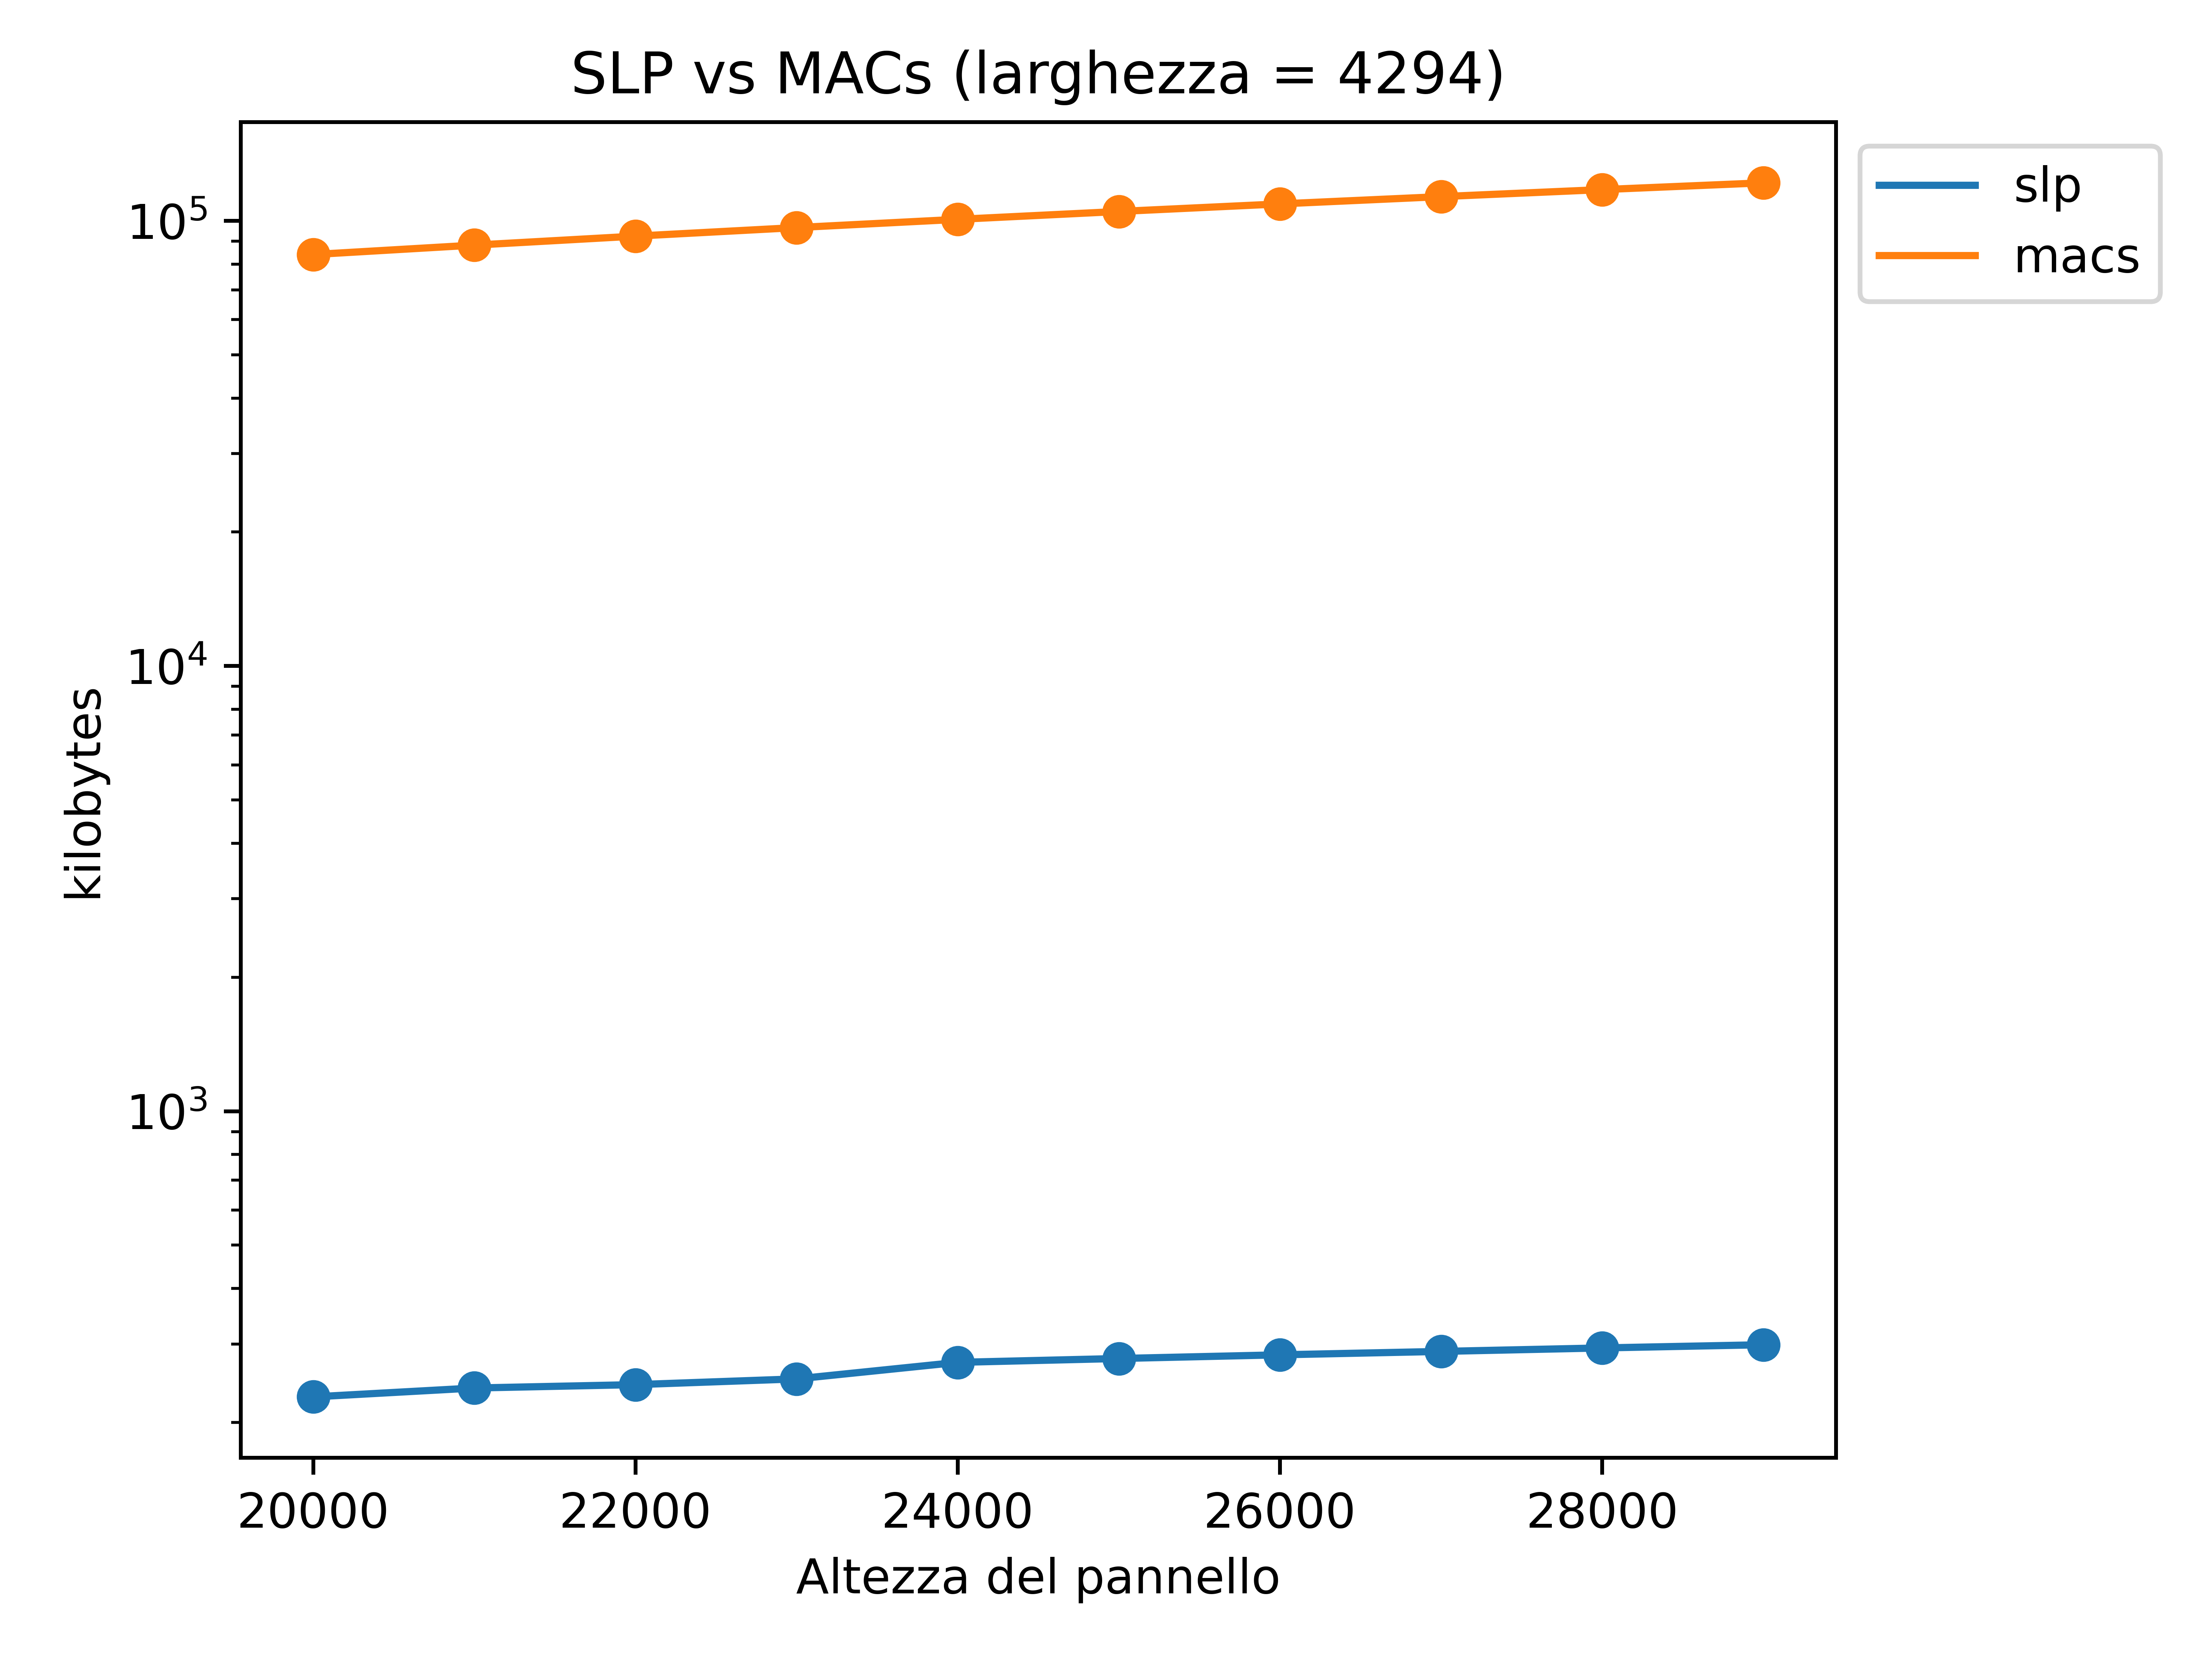
\includegraphics[width=\linewidth]{img/slp_vs_macs.png}
  \end{subfigure}%
  \begin{subfigure}{.5\textwidth}
    \centering
    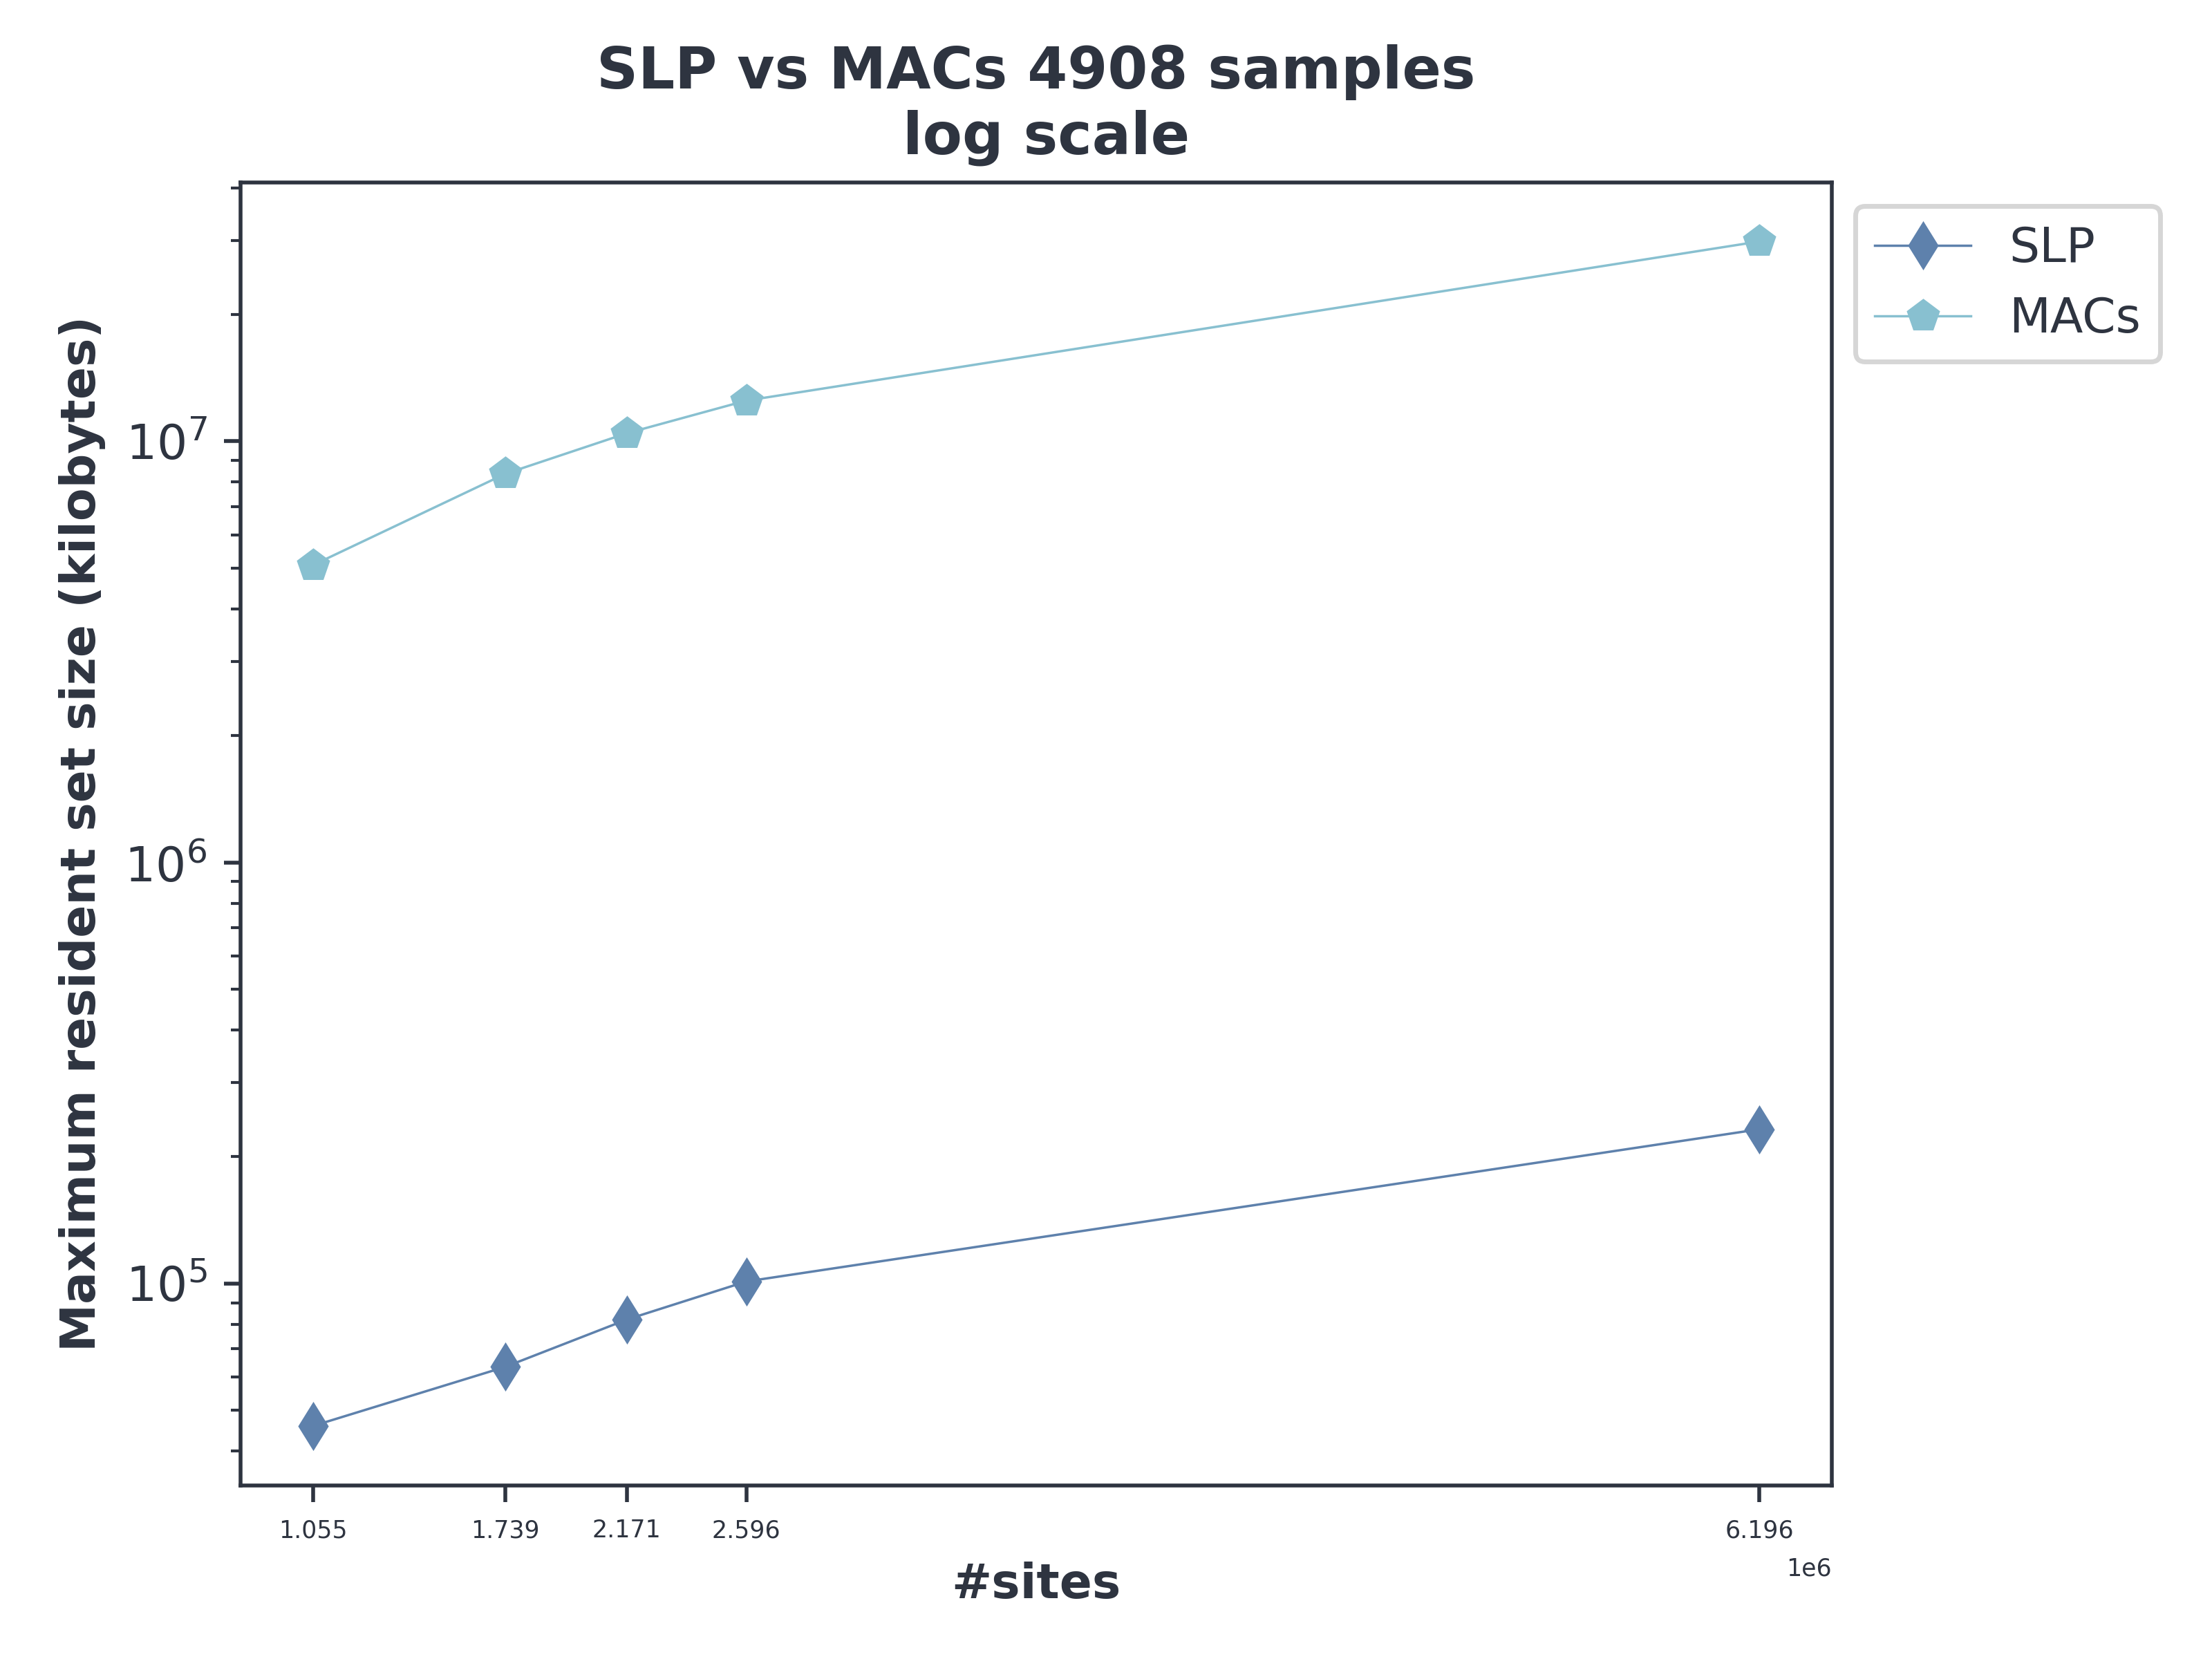
\includegraphics[width=\linewidth]{img/slp_vs_macs_log.png}
  \end{subfigure}
  \caption{Confronto tra la memoria richiesta dai file MACs e dagli SLP per i
    pannelli del 1000 Genome Project. Il grafico di destra è in scala
    logaritmica.} 
  \label{fig:slpmacschr}
\end{figure}
\paragraph{Costruzione della struttura}
Passiamo ora ad analizzare tempi e picchi di memoria per la costruzione delle
strutture dati. Bisogna ricordare che:
\begin{itemize}
  \item nel caso della \textit{RLPBWT} questa fase prevede la costruzione e la
  serializzazione dell'intera struttura dati, comprensiva di tutte le
  sottostrutture necessarie al computo degli SMEM
  \item nel caso della \textit{PBWT} questa fase crea unicamente un file
  compresso ``ad hoc'' con le strutture base delle \textit{PBWT}, a partire
  dalla quale, in fase di calcolo degli \textit{SMEM}, verranno calcolati anche
  tutte le altre strutture necessarie al calcolo degli stessi
\end{itemize}
Fatte queste doverose premesse passiamo ad analizzare i risultati.
In figura \ref{fig:maketimememchr} (a) vengono visualizzati i picchi di
memoria 
richiesti. Anche in questo caso si hanno varie osservazioni possibili:
\begin{itemize}
  \item come anticipato la PBWT non calcola e memorizza tutti gli indici
  necessari al calcolo degli SMEM in fase di costruzione, avendo quindi una
  bassissima richiesta di memoria in questa fase
  \item le strutture \texttt{MAP-INT + LCP} e \texttt{MAP-BV + LCP}, dovendo
  memorizzare l'intero insieme degli \textit{array LCP}, hanno un elevato
  consumo di memoria
  \item confrontando le strutture dati in grado di computare l'array $MS$ si
  nota come le differenze siano relative all'uso o meno dell'\textit{SLP} e
  all'uso o meno delle \textit{threshold}
\end{itemize}
In figura
\ref{fig:maketimememchr} (b), si hanno i tempi di calcolo della costruzione
delle strutture dati. Si possono fare varie osservazioni:
\begin{itemize}
  \item tutti gli algoritmi di costruzione sono in tempo proporzionale a
  $\mathcal{O}(NM)$ ma, come detto, le varianti della \textit{RLPBWT} includono
  in questa fase anche il calcolo delle strutture utili al calcolo degli SMEM
  \item 
  la struttura \texttt{MAP-BV + THR-BV + RA-BV, + PERM + PHI}
  richiede più tempo in quanto deve memorizzare effettivamente il pannello e
  costruire le strutture per \textit{rank/select} dei vari bitvector
  \item la struttura \texttt{MAP-INT + LCE + PERM + PHI}, non dovendo costruire i
  \textit{bitvector sparsi}, le strutture a supporto per \textit{rank/select} e
  il pannello con la componente \texttt{RA-BV}, risulta, in termini di tempi di
  costruzione, 
  essere la più performante parlando delle soluzioni run-length encoded
\end{itemize}
\begin{figure}
  \centering
  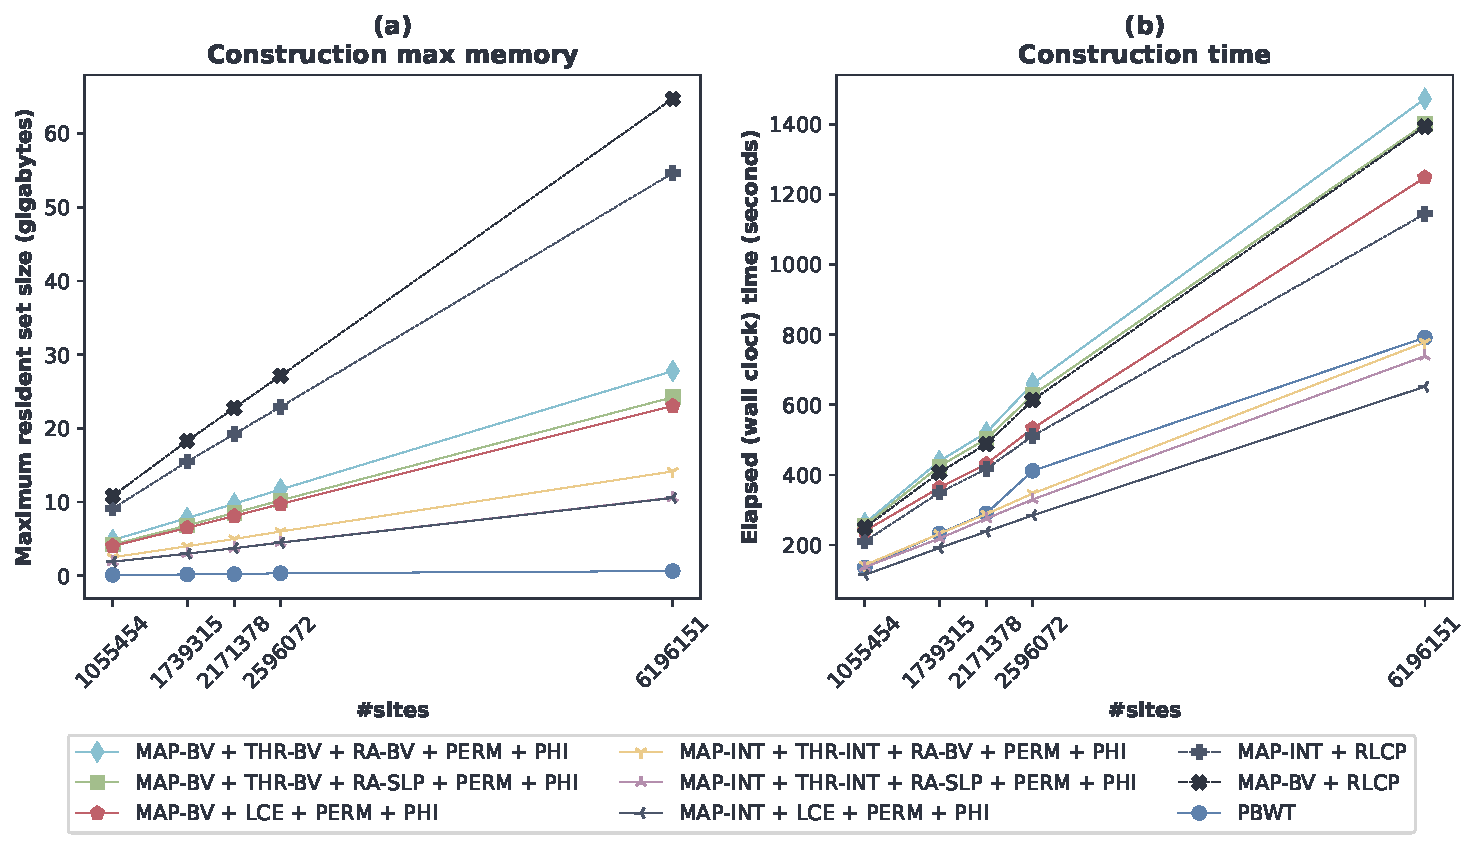
\includegraphics[width=\linewidth]{img/make_time_mem_paper}
  \caption{Picchi di memoria (a) e tempi di esecuzione (b) per  la
    costruzione delle varianti della RLPWBT e per 
    la PBWT.}
  \label{fig:maketimememchr}
\end{figure}
In tabella \ref{tab:comp} si riportano, in megabytes, le dimensioni delle
singole strutture dati che compongono le varianti della \textit{RLPBWT}. Le
stesse misurazioni sono visualizzabili anche in figura \ref{fig:comp}. Si può
innanzitutto apprezzare il vantaggio dell'uso dell'\textit{SLP} rispetto al
pannello non compresso in memoria. Si può notare, inoltre, come il peso dei
bitvector sparsi per le teste di run e le threshold sia pressoché identico. Si
segnala, infine, come memorizzare i \textit{prefix array samples} e la struttura
di supporto per il calcolo delle funzioni $\varphi$ e $\varphi^{-1}$, non
presenti particolari criticità dal punto di vista della memoria richiesta.
\dc{Serve altro?}
\begin{figure}
  \centering
  \begin{subfigure}{.5\textwidth}
    \centering
    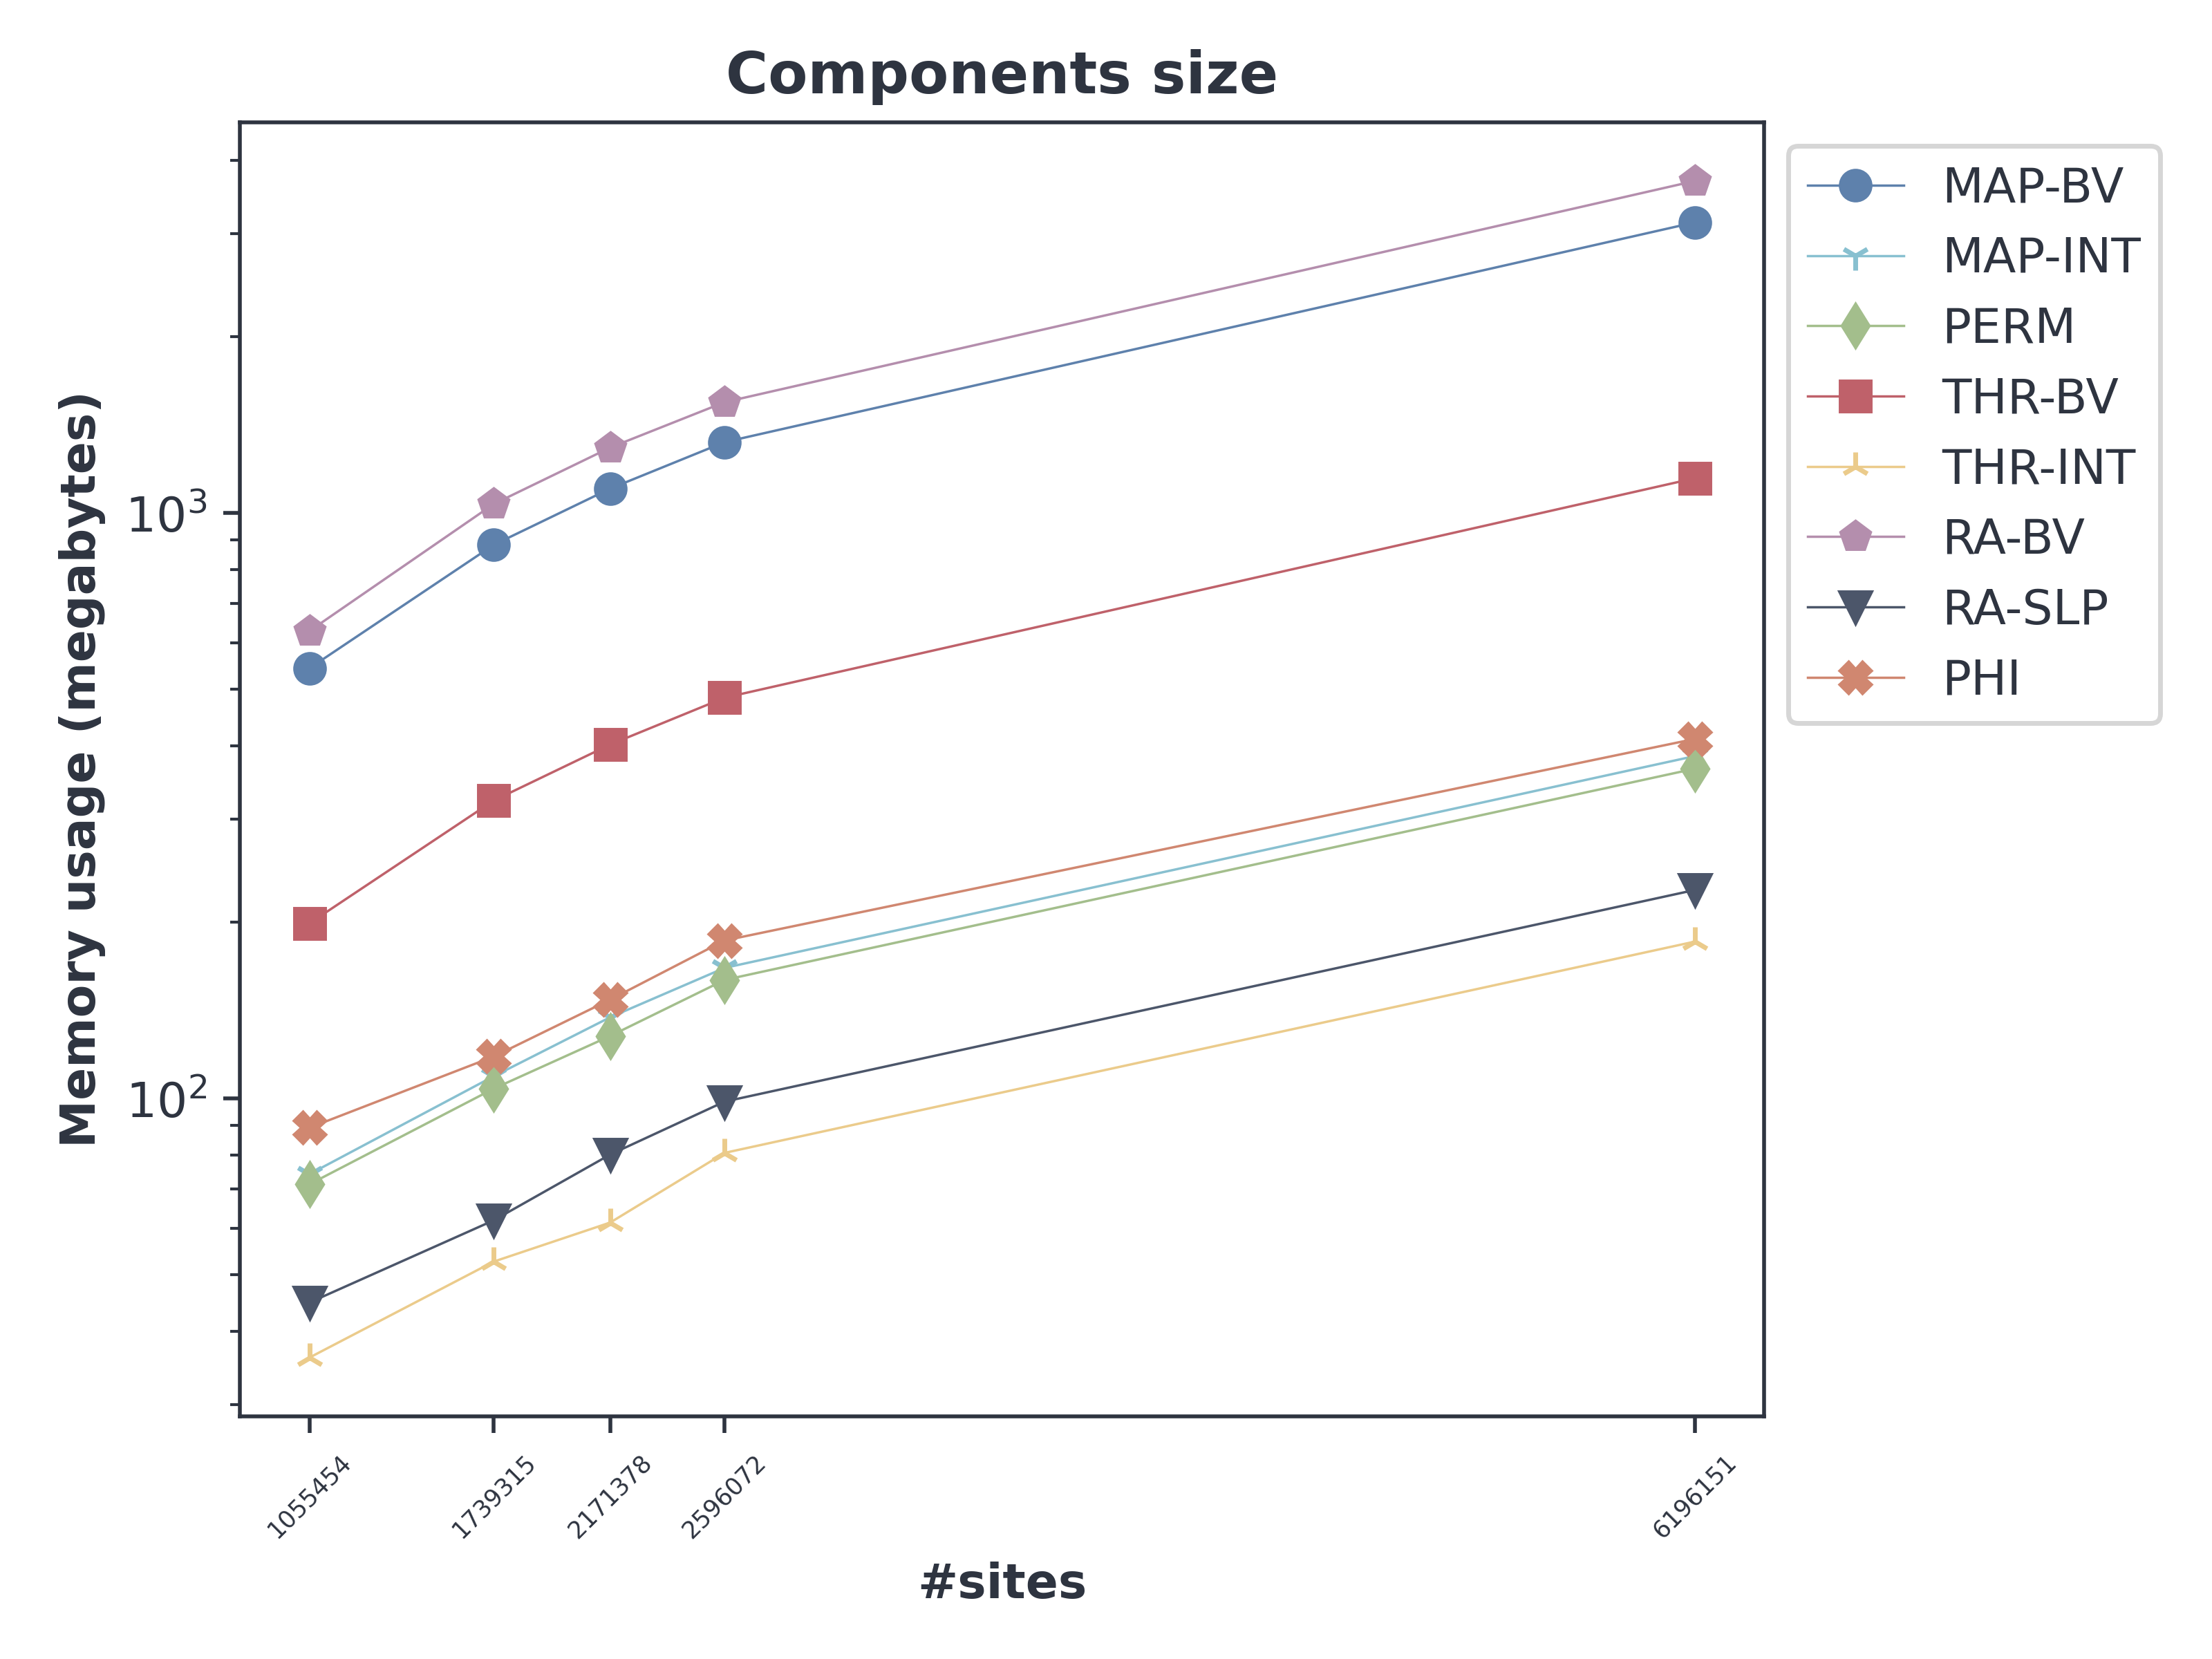
\includegraphics[width=\linewidth]{img/comp_sites.png}
  \end{subfigure}%
  \begin{subfigure}{.5\textwidth}
    \centering
    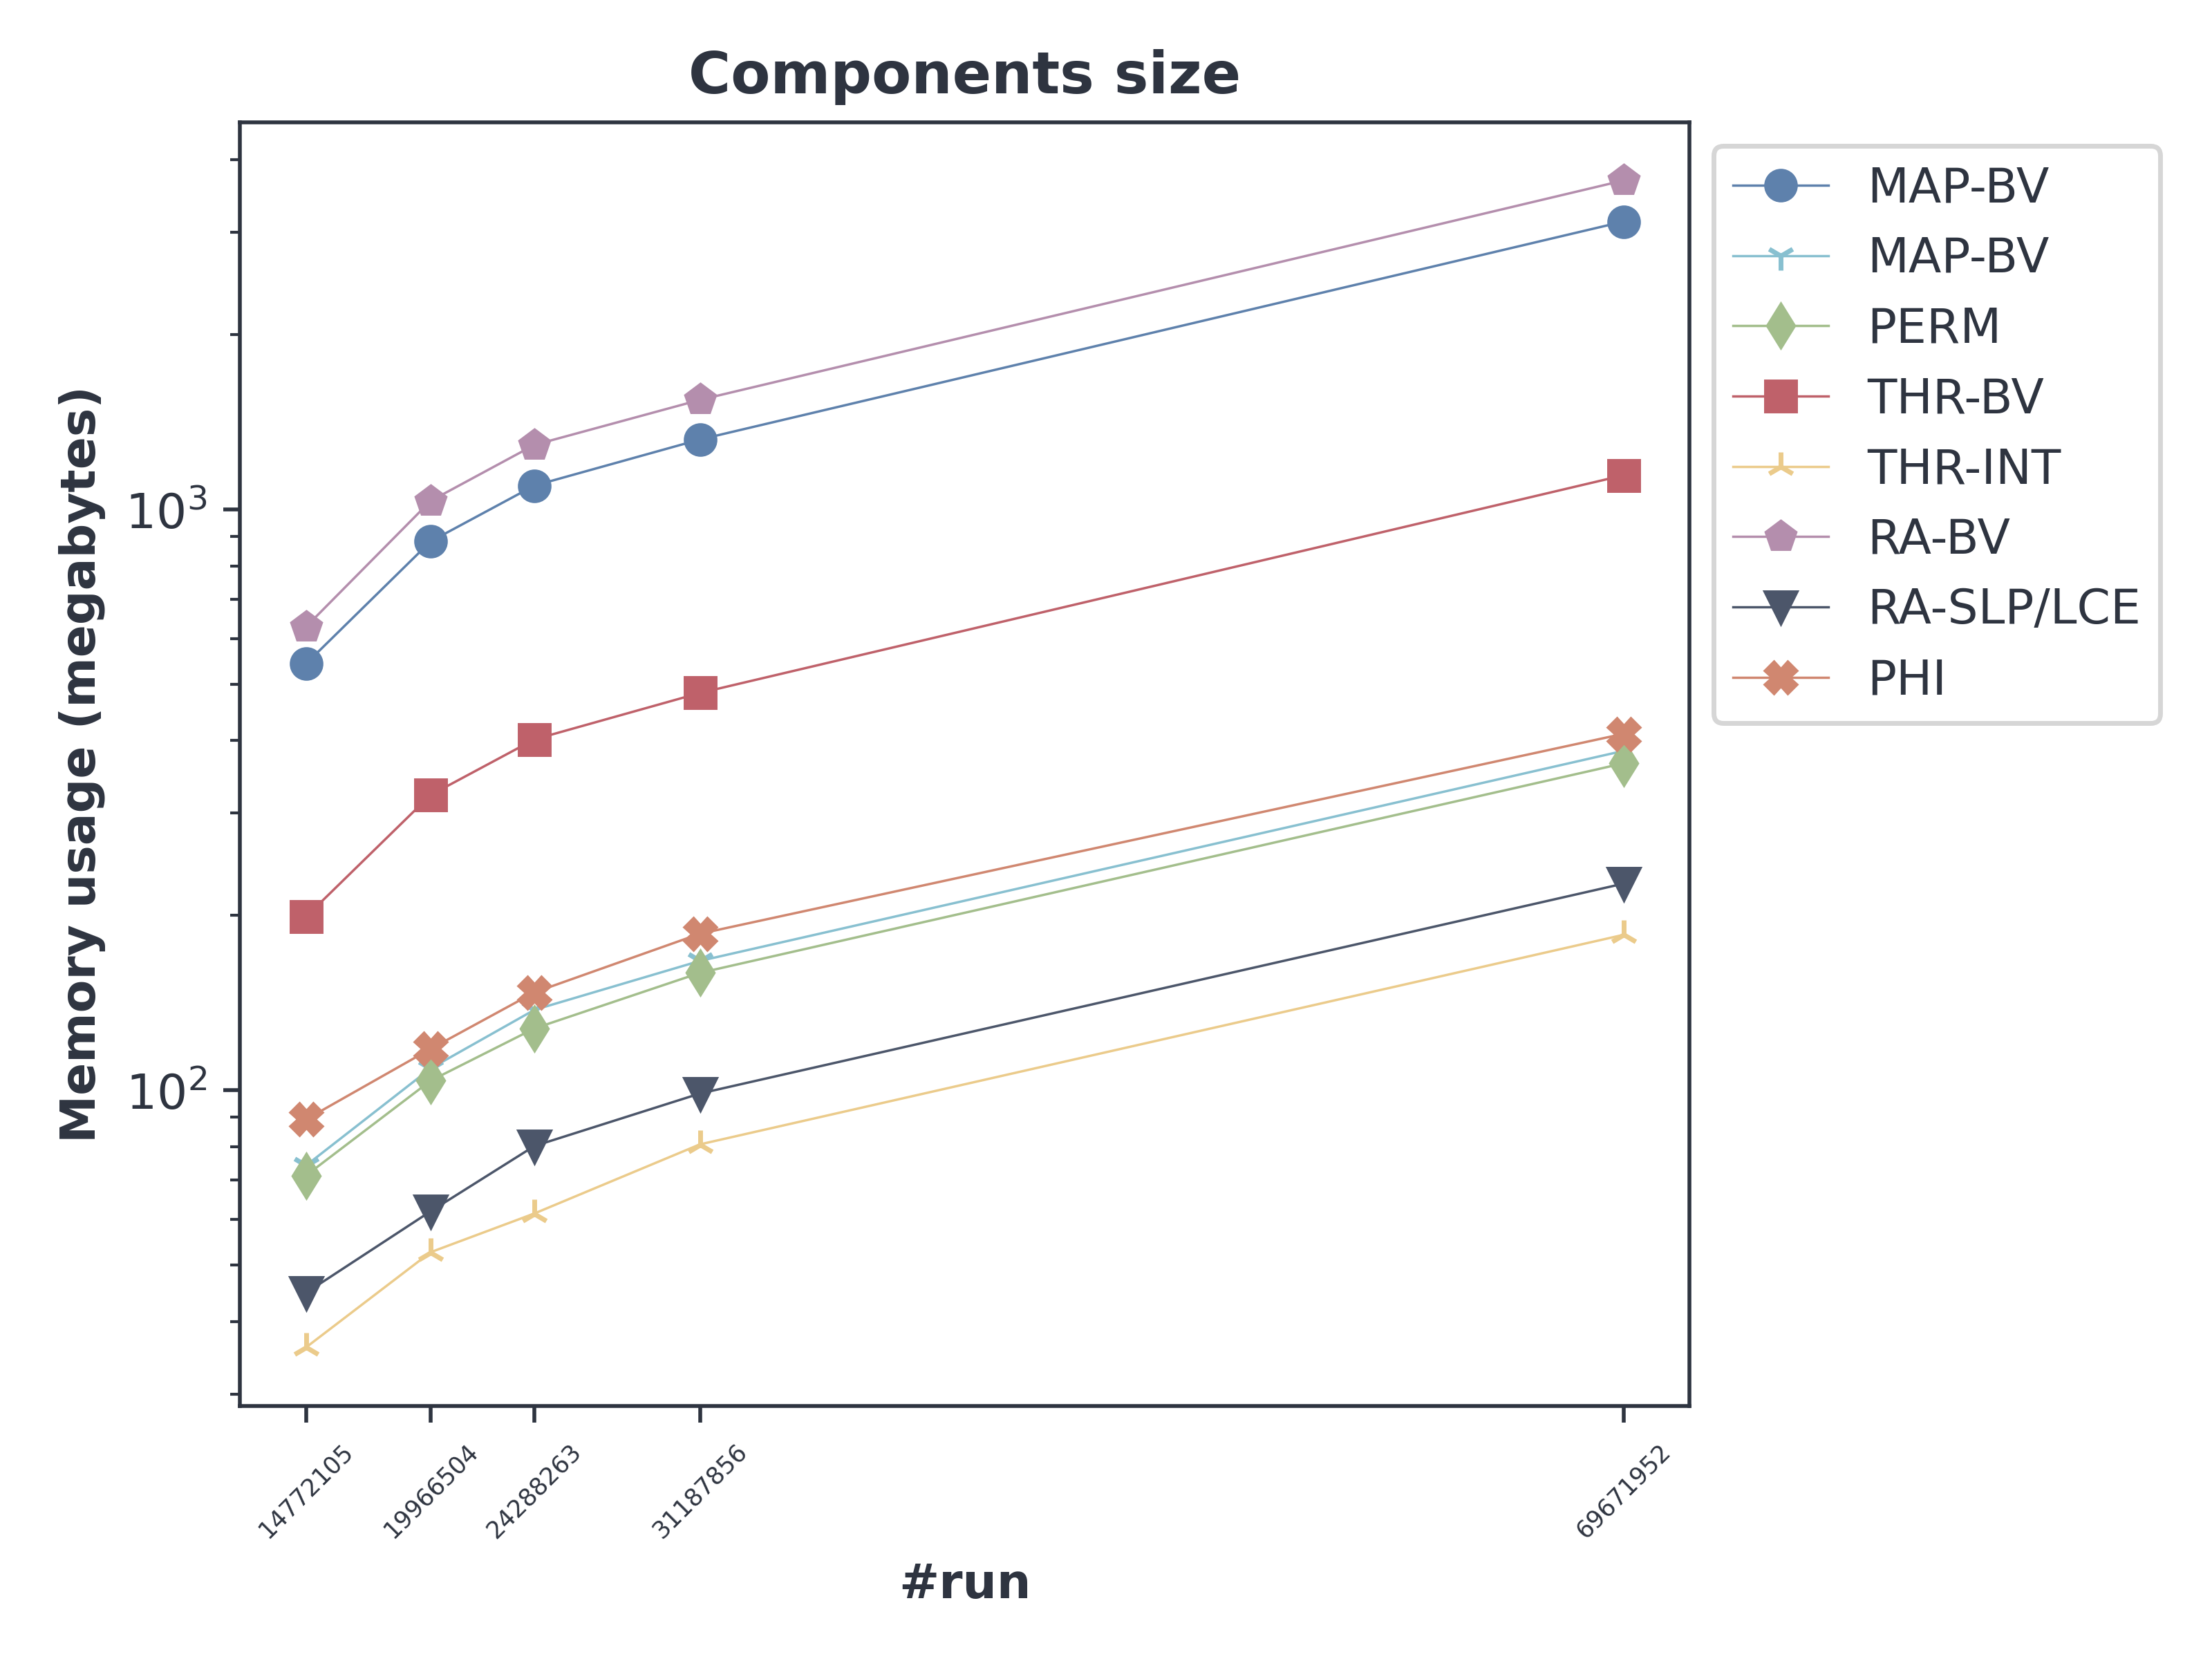
\includegraphics[width=\linewidth]{img/comp_runs.png}
  \end{subfigure}
  \caption{Memoria occupata dalle singole componenti, avendo sulle ascisse sia
    il numero di siti, a sinistra, che il numero di run, a destra. Si noti che
    con \texttt{MAP} si intende $h+u+v+c+start$ mentre con \texttt{THR} $t$. }
  \label{fig:comp}
\end{figure}
\begin{table}
  \centering
  \caption{Dimensioni, in megabytes, delle varie componenti della
    \textit{RLPBWT}.} 
  \label{tab:comp}
  \scriptsize
  \begin{tabular}{c||c|c|c|c|c|c|c|c|c}
    \textbf{Chr}  & \textbf{\textit{t}} & \textit{\textbf{Samples}} & $\boldsymbol\phi$ &
                                                                                 \textbf{SLP}
    & \textbf{Pannello} & \textbf{\textit{h}} &  \textbf{\textit{u}}  &
                                                                        \textbf{\textit{v}}
    &  \textbf{\textit{c}} +  \textbf{\textit{start}}\\ \hline    \hline
    \textbf{22}  & 198.9 & 71.3 & 89.0 & 44.7 & 628.1 & 194.5 & 180.2 & 162.7 & 5.1
    \\ \hline
    \textbf{20}  & 322.5 & 103.8 & 117.9 & 61.9 & 1035.1 & 315.1 &  293.5 & 264.7 & 8.3
    \\ \hline
    \textbf{18}  & 401.9 & 127.8 & 147.4 & 80.2 & 1292.2 & 392.9 & 366.1 & 330.4 & 10.3
    \\ \hline
    \textbf{16}  & 483.4 & 159.3 & 186.1 & 98.7 & 1544.9 & 472.4 & 439.5 & 396.1 & 12.4
    \\ \hline
    \textbf{1}  & 1145.6 & 365.6 & 410.9& 226.9 & 3687.3 & 1119.6 & 1043.4 & 940.4 & 29.5
    \\ 
  \end{tabular}
\end{table}
% \begin{table}
%   \centering
%   \caption{Dimensioni, in megabytes, delle varie componenti della
%     \textit{RLPBWT}.} 
%   \label{tab:comp}
%   \scriptsize
%   \begin{tabular}{|c|c|c||c|c|c|c|c|c|c|c|c|}
%     \hline
%     Chr & Sites & Runs & h+u+v & t & samples & $\phi$ & slp & panel & h & u
%     & v \\ \hline
%     22 & 1055454 & 14772105 & 537.4 & 198.9 & 71.3 & 89.0 & 44.7
%        & 628.1 & 194.5 & 180.2 & 162.7 \\ \hline
%     20 & 1739315 & 19966504 & 873.2 & 322.5 & 103.8 & 117.9
%                                                       & 61.9 & 1035.1 & 315.1 & 293.5 & 264.7 \\ \hline
%     18 & 2171378 & 24288263 & 1089.298 & 401.9 & 127.8 & 147.4
%                                                       & 80.2 & 1292.2 & 392.9 & 366.1 & 330.4 \\ \hline
%     16 & 2596072 & 31187856 & 1307.931 & 483.4 & 159.3 & 186.1
%                                                       & 98.7 & 1544.9 & 472.4 & 439.5 & 396.1 \\ \hline
%     1 & 6196151 & 69671952 & 3103.508 & 1145.6 & 365.6 & 410.9
%                                                       & 226.9 & 3687.3 & 1119.6 & 1043.4 & 940.4 \\ \hline 
%   \end{tabular}
%\end{table}
\paragraph{Calcolo degli SMEM}
Passando all'effettivo calcolo degli SMEM, si possono, anche in questo caso,
confermare i risultati avuti con i pannelli simulati.\\
In figura \ref{fig:smemtimememchr} (a) si riportano i risultati i termini di
picchi di 
memoria durante la computazione degli SMEM. Anche in questo caso, si possono fare
diverse osservazioni:
\begin{itemize}
  \item come previsto, la \textit{PBWT Dynamic} ha le migliori prestazioni anche
  in spazio, calcolando dinamicamente i vari indici per il computo dei match
  massimali interni al pannello
  \item l'\textit{algoritmo 5} di Durbin conferma le previsioni fatte
  dall'autore, avendo che la memoria utilizzata è circa $13NM$ bytes
  \item la differenza tra le varie strutture dati che supportano il calcolo
  dell'array $MS$ è dovuta, a parità di componente per il mapping (e
  conseguentemente della componente per le threshold), dall'uso della componente
  \texttt{RA-BV} o della componente \texttt{RA-SLP}, avendo che la prima
  richiede maggior memoria. All'aumentare delle dimensioni del
  pannello, d'altro canto, si prevede che l'uso dell'\textit{SLP} garantisca
  sempre più un minor uso di memoria
\end{itemize}
% Interessante è notare il rapporto tra la memoria richiesta dalla \textit{RLPBWT}
% con \textit{SLP} e \textit{LCE} e la \textit{PBWT Indexed}:
% \begin{table}[H]
%   \centering
%   \footnotesize
%   \begin{tabular}{c|c|c|c|c}
%     \textbf{\#Samples} & \textbf{\#Siti}
%     & \textbf{RLPBWT SLP-LCE (\textit{kb})}
%     & \textbf{PBWT Indexed (\textit{kb})} & \textbf{\%}\\
%     \hline
%     4908 & 1055454 & 3058088 & 65975520 & 4.64\\
%     4908 & 1739315 & 4961664 & 108713424 & 4.56\\
%     4908 & 2171378 & 6190684 & 135726084 & 4.56\\
%     4908 & 2596072 & 7430300 & 162257008 & 4.58\\
%     4908 & 6196151 & 17635700 & 387252160 & 4.55
%   \end{tabular}
% \end{table}
% Anche in questo caso le percentuali risultano leggermente peggiori rispetto ai
% pannelli simulati, pur restando risultati molto interessanti.
In figura \ref{fig:smemtimememchr} (b) si riportano i risultati i termini di tempo di
calcolo, notando che:
\begin{itemize}
  \item come atteso, l'algoritmo \textit{PBWT Dynamic} risulta essere il più
  performante
  \item la struttura \texttt{MAP-INT + THR-INT + RA-SLP + PERM + PHI} e la
  struttura 
  \texttt{MAP-BV + THR-BV + RA-SLP + PERM + PHI}, a causa dei
  frequenti accessi all'\textit{SLP}, sia per il calcolo delle lunghezze delle
  matching statistics che per la fase di ``disambiguazione'', richiede più tempo
  di tutte le altre varianti, soprattutto se si pensa alla corrispondente
  variante senza \textit{SLP}
  \item la struttura \texttt{MAP-INT + LCE + PERM + PHI} e la struttura
  \texttt{MAP-BV + LCE + PERM + PHI} risultano essere, al massimo,
  il doppio più lenta della soluzione proposta da Durbin con l'\textit{algoritmo
    5}. Questo è un risultato 
  molto interessante se si tiene in considerazione la memoria necessaria per il
  calcolo degli \textit{SMEM}
\end{itemize}
\begin{figure}
  \centering
  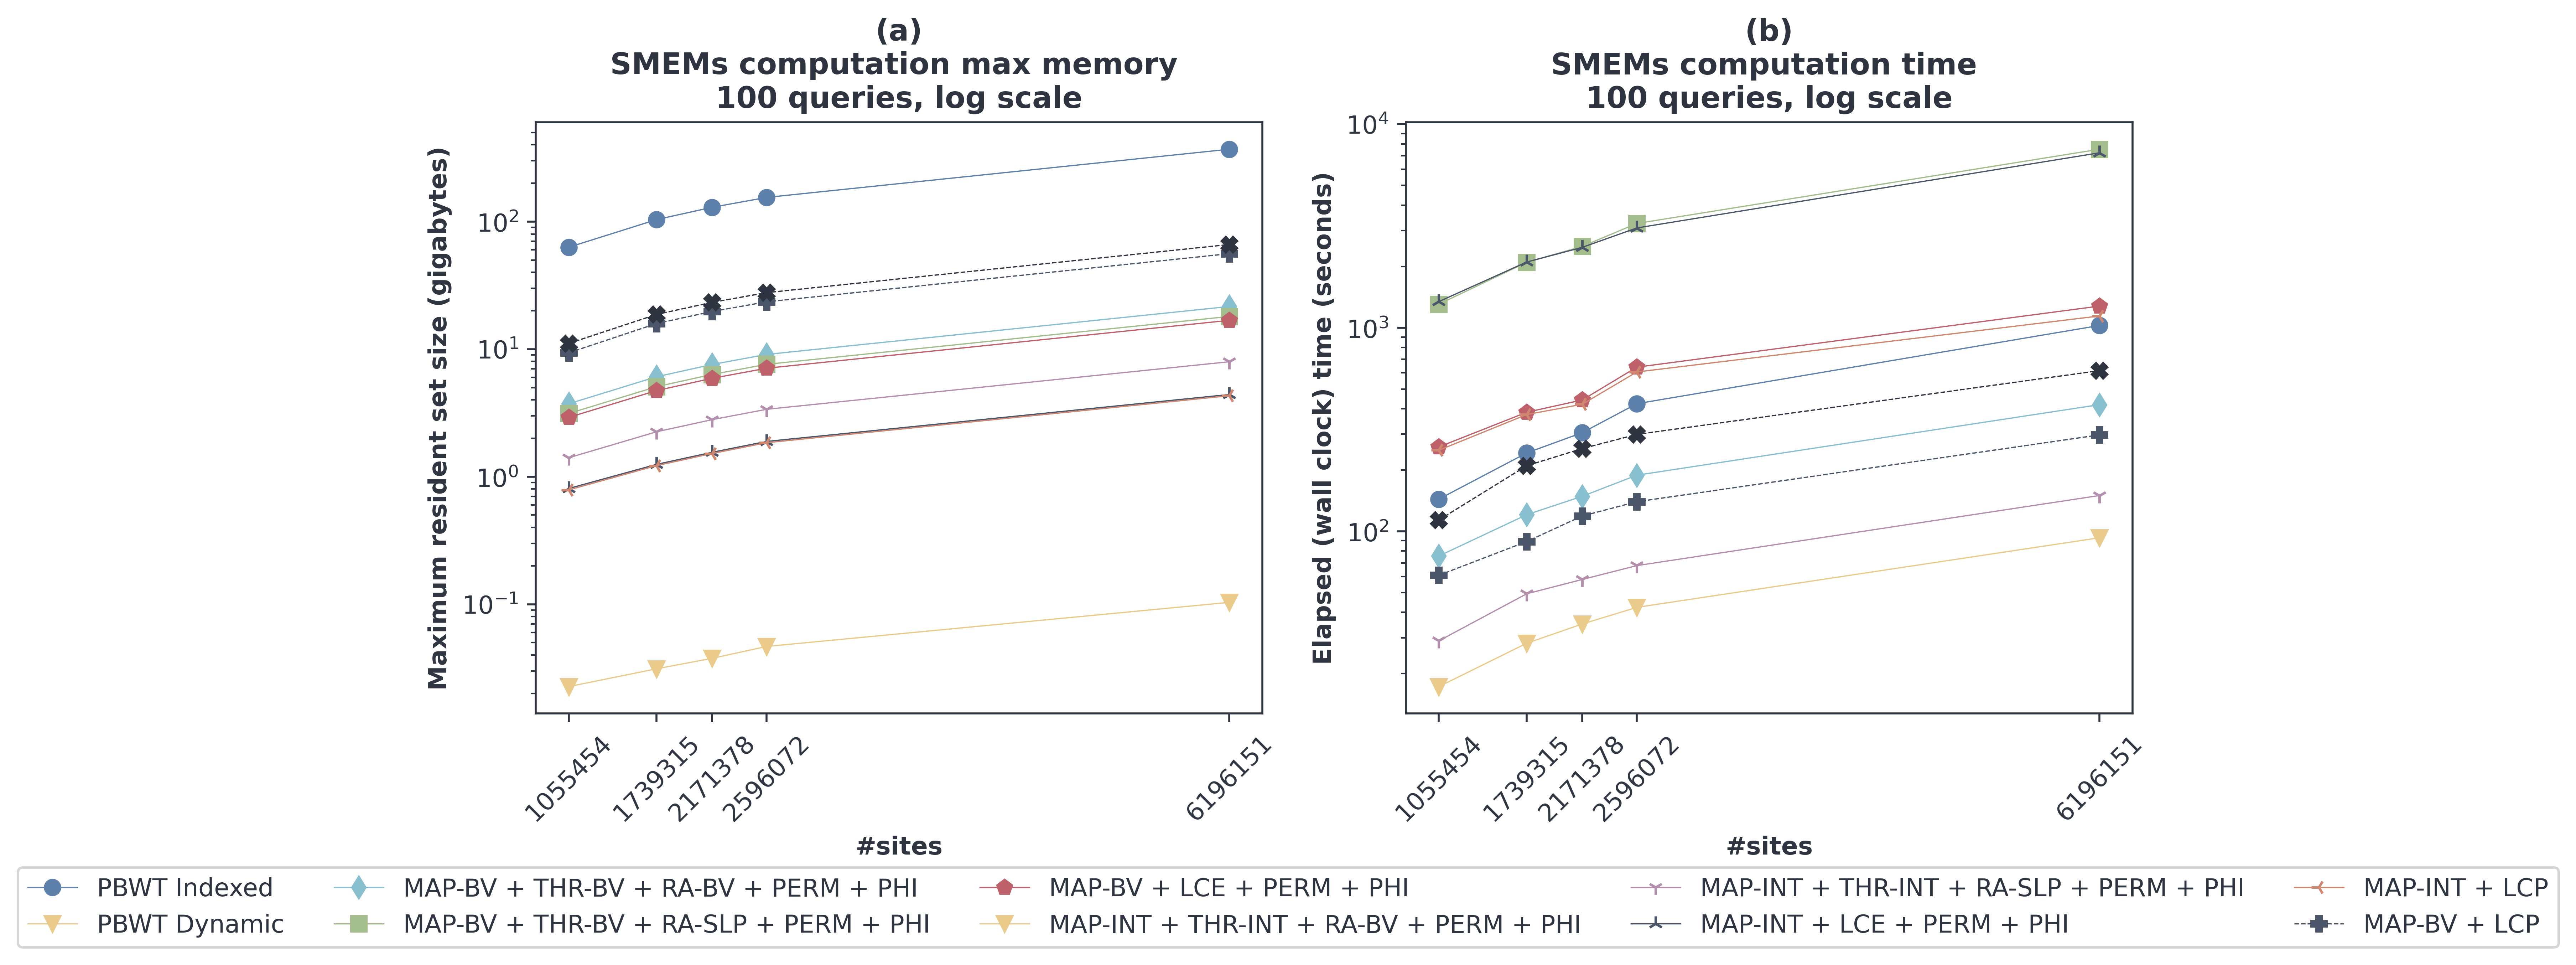
\includegraphics[width=\linewidth]{img/exe_time_mem_paper}
  \caption{Picchi di memoria (a) e tempi di esecuzione (b) per il calcolo degli
    SMEM.}
  \label{fig:smemtimememchr}
\end{figure}
\subsection{Tempo di una singola query}
Infine, per completare lo studio delle prestazioni temporali, si è deciso di
isolare il calcolo degli SMEM con ogni singola query, valutando media e
deviazione standard delle 100 query. Tale risultato è visualizzabile in figura
\ref{fig:smemsinglechr}, dove si è deciso di escludere le strutture
\texttt{MAP-INT + LCP} e \texttt{MAP-BV + LCP} in quanto non in grado di
computare quali righe presentino un certo SMEM, e conferma quanto ipotizzato e
discusso precedentemente: 
\begin{itemize}
  \item la \textit{PBWT Dynamic} richiede di costruire, ogni volta, la
  trasformata della query e
  calcolare i match interni al pannello originale a cui viene
  aggiunta la query, considerando poi solo i match provenienti da tale
  pannello. Questo processo richiede molte operazioni e non è ottimizzato per 
  una singola query. Una query o un centinaio di query hanno quindi all'incirca
  lo tempo di calcolo
  \item la \textit{PBWT Indexed} richiede molto meno operazioni ed è quindi la
  soluzione più performante
  \item per quanto riguarda la \textit{RLPBWT}, con l'uso della componente
  \texttt{RA-SLP}, si rilevano gli stessi problemi relativi all'random access,
  precedentemente 
  descritti. Questi problemi sono risolti con l'uso della componente
  \texttt{RA-BV} 
  \item a parità di componenti per il mapping (e conseguenti componenti per le
  threshold), l'uso della componente \texttt{LCE} risulta più lenta dell'uso
  della componente \texttt{RA-BV}, a causa dei costi di calcolo delle
  \textit{LCE query} stesse 
\end{itemize}
Tali risultati sono ottenuti isolando unicamente le singole funzioni atte al
calcolo dei match, escludendo i tempi di caricamento delle strutture o di
eventuali ulteriori costruzioni (come degli array nel caso della \textit{PBWT
  indexed} o della \textit{PBWT} della singola query nel caso della \textit{PBWT
Dynamic}).
\begin{figure}
  \centering
  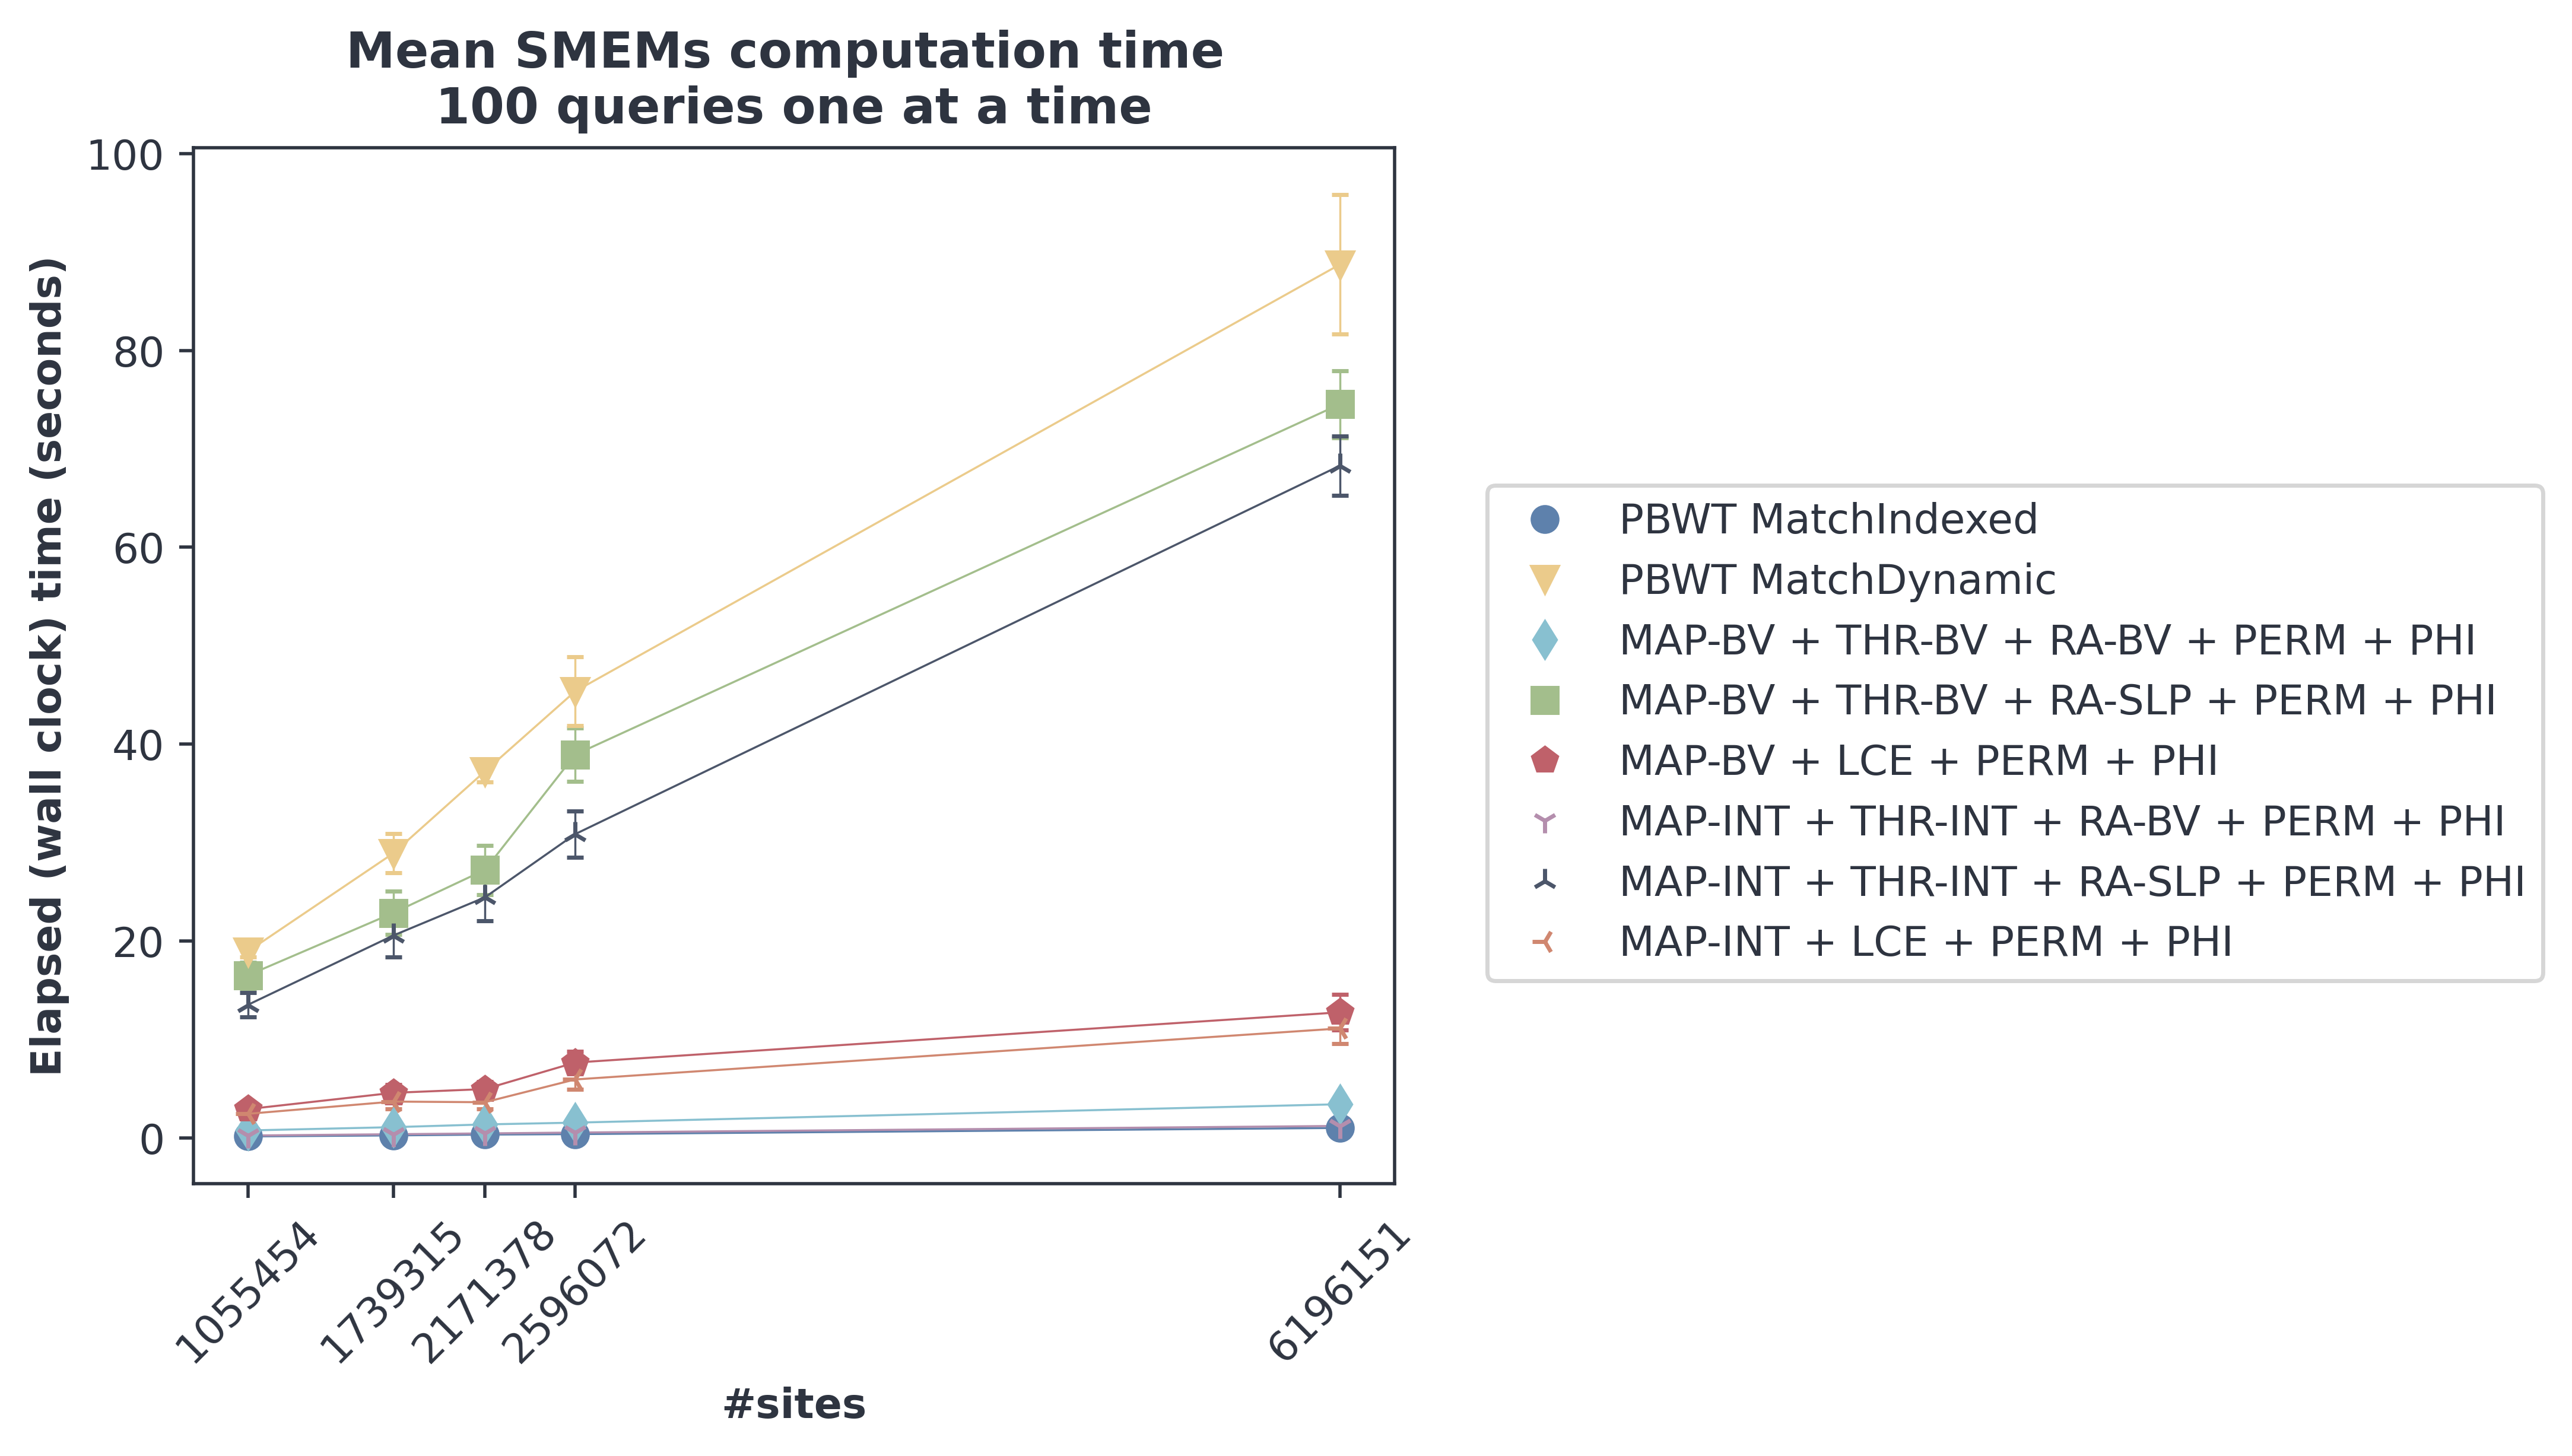
\includegraphics[width=\textwidth]{img/exe_time_single_paper.png}
  \caption{Tempo medio di esecuzione del calcolo degli SMEM per una singola
    query. Il grafico di destra è in scala logaritmica e, in entrambi, le
    barre d'errore rappresentano la deviazione standard.}
  \label{fig:smemsinglechr}
\end{figure}
% LocalWords:  sottostrutture
